\chapter{强化学习概述}
\label{chap:rl-overview}

仓储中的移动机器人要绕开货箱，驶向指定的停靠区。前进还是转向，既影响当前的位置，也影响下一步还能走哪些路线。我们可以让机器人每一步都尽量靠近目标，但这条规则可能使它在障碍前反复试探，或者进入难以脱身的位置。当前一步走得近，不等于整段行动能完成任务。要选择动作，我们需要把动作引起的环境变化与此后的结果一起考虑。

\term{强化学习}（reinforcement learning, RL）研究怎样根据行动后得到的反馈学习决策规则。学习者尝试一种行动，观察结果，再调整以后的选择；调整所依据的目标是长期累计收益，而不只是当前一步的评分。反馈可以是收益，也可以是代价。图~\ref{fig:rl-overview-embodied-setting}~中的机器人展示了这种交互：动作改变场景，新场景又成为下一次决策的依据。

为了逐步核算这些关系，我们把仓储场景简化成一个带障碍和随机滑移的网格任务，并围绕四个彼此衔接的问题展开本章。首先要描述清楚：在什么位置可以提交哪些命令，命令执行后位置和场景按什么规律变化，这就是状态、动作与环境规律要回答的问题。其次要规定决策规则本身：到达每个位置时究竟怎样在允许的命令之间作选择，这样的规则称为策略。再次要规定计分方式：怎样把每一步得到的即时反馈合成为一个能够衡量整段行动好坏的总分，这涉及奖励与累计回报。最后，在真正行动之前就要比较不同命令可能带来的长期结果，用于这种比较的量称为价值。

这四个问题还通过一条线索连在一起：策略不仅决定当前得分，还决定机器人接下来会到达哪些位置、看到哪些情况，因而决定以后能够收集到什么样的行动记录。评价一条规则有多好，与说明交互训练记录是按什么规则产生的，因此是同一个问题的两面，不能分开处理。本章先用概率、条件期望与基础优化知识把这四个对象讲清楚；至于给定规律后如何高效算出价值、规律未知时如何从交互记录中估计价值，分别由后续两章展开。

\begin{figure*}[htbp]
  \centering
  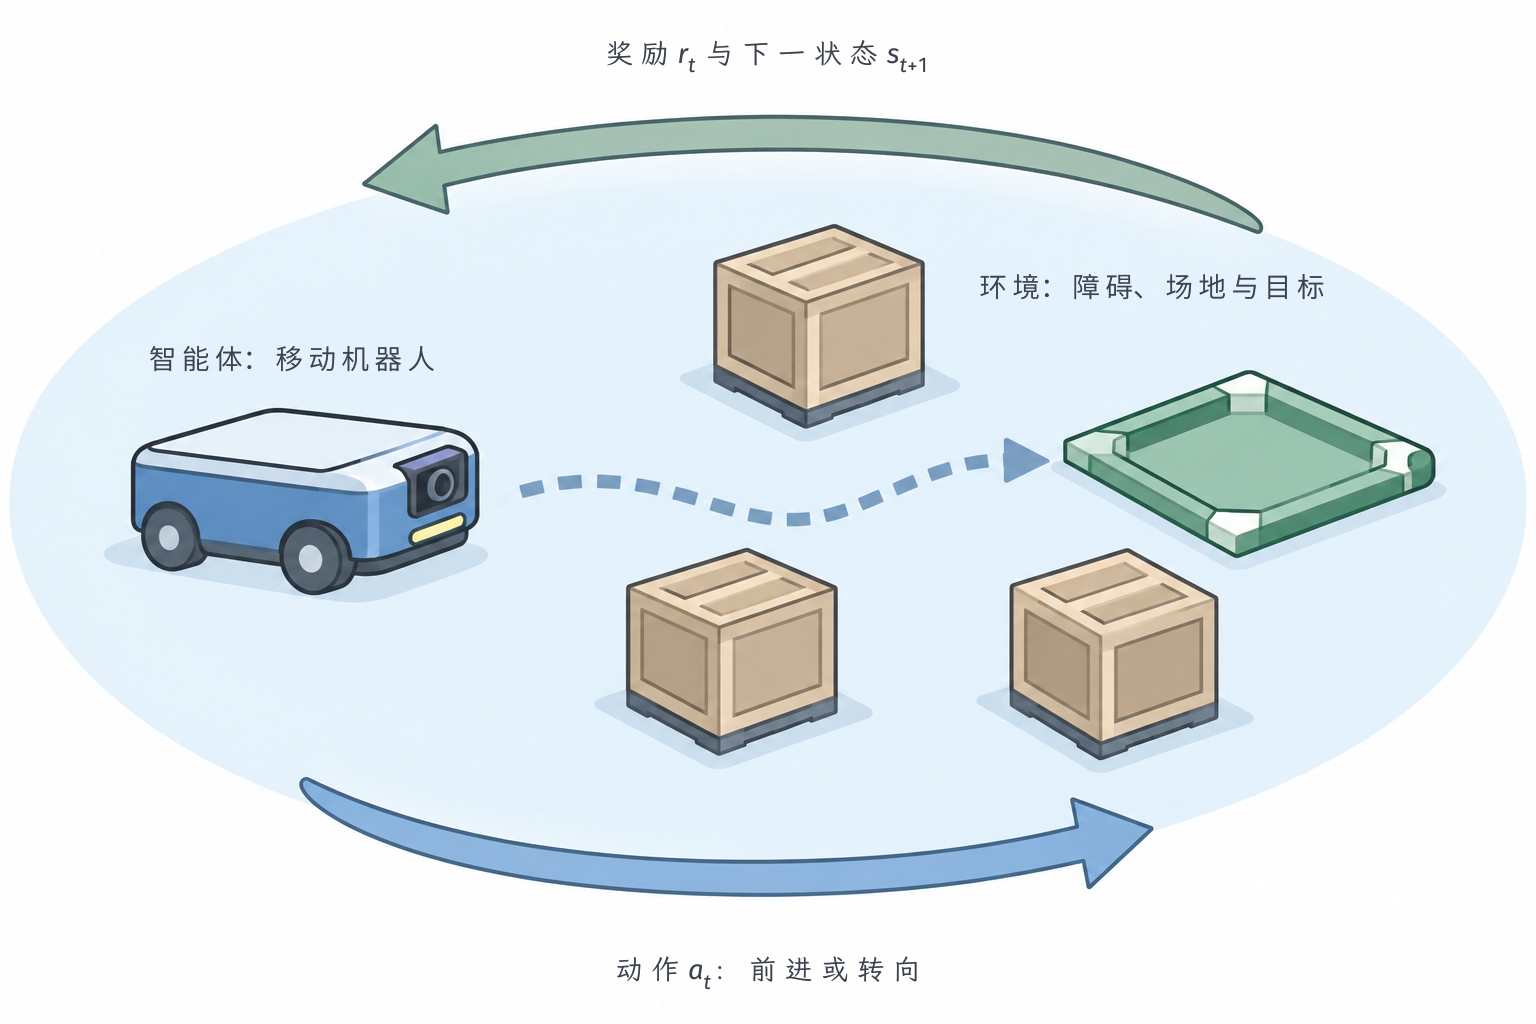
\includegraphics[width=157.400mm]{figures/07-reinforcement-learning/01-problems-and-solving/generated/rl-overview-embodied-loop/figure.png}
  \caption{完全可观测教学设定中的具身交互。移动机器人能够取得当前状态，据此选择动作；环境执行动作后改变场景，并返回奖励和下一状态。一般任务中机器人取得的是观测，观测未必揭示完整状态。插图只表达交互关系，不表示精确动力学、传感器结构或实验结果。}
  \label{fig:rl-overview-embodied-setting}
\end{figure*}

% Outline: 1.1
\Needspace{35mm}
\section{强化学习的基本设定}
\label{sec:rl-overview-setting}

% Outline: 1.1.1
\subsection{智能体与环境的交互}
\label{sec:rl-overview-interaction}

在仓储任务中，机器人可以提交前进、转向或停止等命令，却不能直接指定命令执行后的精确位置。地面摩擦、货箱位置和执行误差也会影响实际运动。我们把选择命令的主体称为\term{智能体}（agent），把命令给定后产生运动和反馈的过程称为\term{环境}（environment）。这种划分明确了学习算法能够改变的是命令选择规则，而不是任意改变物理后果。到达停靠区可以得到正奖励，碰撞或耗时可以产生代价；这些评分怎样共同评价任务，还需要另行规定。

为预测命令执行后的变化，需先规定用哪些变量描述当前环境。状态（state）是用于预测后续变化的环境描述，记为$s_t$；机器人的位置、朝向和障碍物位置可以共同组成一个状态。\term{状态空间}（state space）$S$收集任务中所有可能的状态，也就是这些变量在任务内允许出现的组合。动作$a_t$表示一次具体命令，\term{动作空间}（action space）$\mathsf A$则收集所有命令形式；这里的“动作”与前卷的“行动”指同一对象。命令可能只在某些状态下可执行，状态$s$下允许的命令组成$\mathsf A(s)\subseteq\mathsf A$。

环境状态与智能体实际取得的观测未必相同。观测（observation）是传感器或交互接口给出的测量结果，记为$o_t$：机器人的位置可以属于状态，相机拍到的局部图像则是观测。一张图像可能遮住了影响运动的障碍，因而不足以预测下一步。下面先假设智能体能够直接读出完整状态，即$o_t=s_t$，再将一次命令及其后果组成交互记录。

\begin{definition}[智能体、环境与一步经验]
  \label{def:rl-overview-interface}
  设$S$为状态集合，$\mathsf A$为动作集合，$\mathsf A(s)\subseteq\mathsf A$为状态$s$下非空的允许动作集合。离散时刻$t=0,1,\ldots$的状态为$s_t\in S$，所选动作为$a_t\in\mathsf A(s_t)$。智能体是依据可得观测和历史选择动作的主体，环境是在动作给定后产生后继状态与反馈的过程。在完全可观测（fully observable）设定下，观测$o_t=s_t$。执行$a_t$后取得奖励$r_t\in\mathbb R$和后继状态$s_{t+1}$，四元组
  \[
    (s_t,a_t,r_t,s_{t+1})
  \]
  称为一步经验，也称一步交互记录。$r_t$按动作发生的时刻编号，表示执行$a_t$之后得到的反馈。
\end{definition}

决策历史记为$I_t$，由行动前已取得的观测、过去动作及可见奖励组成。智能体只能利用当时已经取得的这些记录选择动作，不能读取尚未发生的奖励。本章先取$o_t=s_t$，不完整观测下怎样利用$I_t$由第~\ref{chap:rl-information}章处理。状态、观测与决策依据的区分沿用前卷的共同学习框架，可参考\BookChapterRef{chap:mathematics-and-future-research}{卷2《数学准备：概率、因果与决策》中讨论数学基础与后续研究的章节}。

我们用网格位置作为状态，把上述接口缩小到一个可以手算的任务。网格宽$4$、高$3$，坐标为$x=1,\ldots,4$、$y=1,\ldots,3$；起点为$(1,1)$，终点为$(4,3)$，障碍$(2,2)$不可进入。到达终点的那一步得$1$，其余非终止步得$-0.04$。这些数值是教学假设，不是实验测量。方向命令可能因滑移而执行偏离，因此下面三条记录可以依次发生：
\[
\begin{aligned}
 &((1,1),\text{右},-0.04,(2,1)),\\
 &((2,1),\text{右},-0.04,(2,1)),\\
 &((2,1),\text{右},-0.04,(3,1)).
\end{aligned}
\]
第二条记录中，命令仍是向右，位置却没有改变。这可以由滑向障碍或边界造成，不能据此把动作改记为“停留”。经验同时保留命令和结果，才能区分选择规则与执行误差。

取得交互记录以后，学习规则才能据此构造训练目标并调整策略。图~\ref{fig:rl-overview-loop}用实线表示每步执行，用虚线表示记录收集和参数更新：采集器可以每步记录，参数更新却可以每积累一批记录才执行一次。部署时也可以固定参数，只保留执行闭环。因此，交互次数与梯度更新次数需要分别计算。

参与拟合的有限记录组称为训练样本，记为$D=(Z_1,\ldots,Z_n)$。每条$Z_i$可以是一条一步交互记录，也可以是一段完整轨迹；$Z_i$具体表示什么，必须随采集协议一并说明。这里特意保留记录的先后顺序和重复出现：机器人沿一条轨迹连续行动，相邻记录本就相互影响，同一种意外也可能多次发生，因此不能默认这些记录像独立抽签那样互不相关。除训练样本外，还可以按记录的用途划分另外两组：用于在候选规则之间作比较、帮助选择的称为验证样本$D_{\mathrm{va}}$；选择完成后，再用一组没有参与选择的记录独立检验最终规则，称为测试样本$D_{\mathrm{te}}$。训练、验证与测试描述的是同一批可能格式相同的记录被怎样使用，而不是记录来自真实机器人还是仿真程序。

怎样使用训练记录，还取决于允许在哪些行为规则中作选择。考虑一个最简单的情形：暂时只允许在两份事先写好的导航规则之间选择，每份规则在每个状态下都给出合法命令。这两份规则就划定了候选范围；而根据采集到的记录比较二者、并从中选出一份的那套计算过程，则属于选择程序。候选范围回答“可以选什么”，选择程序回答“凭记录怎样选”，两者即使都已确定，也还没有指出某次训练最终会选中哪一份——那要看具体记录与程序中的随机因素。

一般的策略学习也保留同样的层次，只是把候选规则记为策略，把候选范围记为候选策略类$\Pi$。学习规则需要完整规定四件事：允许哪些候选、怎样由训练样本构造比较用的目标、参数怎样初始化和逐步更新、以及何时停止并读出策略。先固定这些规则、训练配置和计算预算，单次拟合所得策略可以记为$\pi_D=A(D,U)$：$A$是从训练样本及随机源到候选策略的学习映射，$U$汇集初始化、抽样等算法随机性。这里$D$是程序使用的有限交互记录组，$A$规定怎样使用这些记录，$\pi_D$是这一次拟合得到的候选策略；某一步实际选出的动作又是执行该策略的结果。训练样本、学习映射、拟合所得策略和执行动作由此分属四个不同层次。

若还要利用验证样本选择超参数或检查点，固定训练样本与拟合随机数就不足以确定最终部署策略。为写清这层依赖，将参与拟合的样本也记为$D_{\mathrm{tr}}=D$，用$\eta\in\Lambda$表示允许选择的训练配置，$A_\eta$表示固定配置后的拟合映射；这些映射给出的候选策略都属于共同的$\Pi$。把拟合与选择使用的随机源合记为$U=(U_{\mathrm{fit}},U_{\mathrm{sel}})$，整个程序可写成
\[
 \widehat\eta=\operatorname{Select}(D_{\mathrm{tr}},D_{\mathrm{va}},U),
 \qquad
 \pi_{\mathrm{final}}
 =A_{\widehat\eta}(D_{\mathrm{tr}},U_{\mathrm{fit}})
 =A_{\mathrm{final}}(D_{\mathrm{tr}},D_{\mathrm{va}},U).
\]
选择规则还须规定怎样比较验证结果和处理并列；若验证结果决定何时停止，停止程序也属于$A_{\mathrm{final}}$。要进一步讨论最终策略的随机分布，还要求选择规则以及$(\eta,D_{\mathrm{tr}},U_{\mathrm{fit}})\mapsto A_\eta(D_{\mathrm{tr}},U_{\mathrm{fit}})$联合可测，从而上述复合程序仍是可测映射。例如，两份候选导航策略在同一训练样本上已经拟合完，另一次验证可能改变它们的回报排序，进而改变部署时选中的策略。执行阶段固定的是全部拟合与选择完成后的$\pi_{\mathrm{final}}$，再依据当前观测或决策历史选择动作，而不能把验证样本对最终结果的影响隐藏在一次固定配置的拟合映射里。

改变规则后，机器人可能进入此前很少经过的区域，新采集的训练记录随之改变分布。常见的监督学习基准分析把训练样本的生成规律视为固定；强化学习则必须额外处理“策略改变后，后续训练样本的分布也跟着改变”这层闭环关系。需要说明的是，监督学习的技术手段仍然可以用于这样的闭环，这里区分的是两类问题设定，而不是把两类技术割裂开来\scite{sutton2018}。

\begin{figure}[htbp]
  \centering
  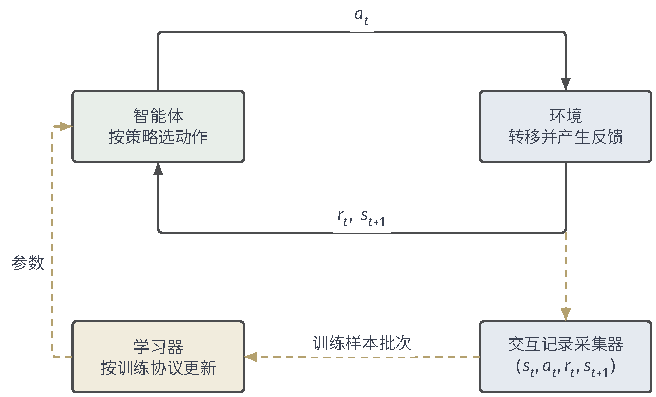
\includegraphics[width=111.100mm]{figures/07-reinforcement-learning/01-problems-and-solving/tikz/rl-overview-loop.pdf}
  \caption{交互与学习的接口。实线是每步执行的动作和反馈，虚线是经验收集及按训练协议发生的参数更新。部署时可移除虚线部分而保留执行闭环。}
  \label{fig:rl-overview-loop}
\end{figure}

% Outline: 1.1.2
\subsection{马尔可夫决策过程}
\label{sec:rl-overview-mdp}

前面三条经验只告诉我们已经发生了什么。它们无法回答一个对决策更关键的问题：如果在同一个位置改选其他动作，结果会怎样？已发生的记录里根本没有这种尝试，因此单凭记录本身无法比较没有执行过的命令。要在行动之前就算出每个选择的可能后果，我们需要一个环境模型：对每个状态和动作，给出它可能导致的下一状态、奖励，以及各种结果出现的概率。

在写出这份模型之前，先引入一个能大幅简化计算的假设。若给定当前状态与动作后，后果的条件分布不再随更早的历史改变，那么预测这一步时就无需翻出过去的观测、动作和奖励，只需知道现在处在哪个状态、准备执行什么命令。这一条件称为马尔可夫性（Markov property）。它不是在断言“真实世界没有历史”，而是在要求所选状态已经概括了过去观测、动作与奖励记录中预测下一步后果所需的部分；它的实际好处是让我们能够始终从当前状态开始向前计算，而不必逐次重放整段经历。

把这样的转移规律与可选动作结合，就得到\term{马尔可夫决策过程}（Markov decision process, MDP）。顾名思义，它是一个“做决策”的过程：描述智能体在哪些状态可以选哪些动作，以及每次选择之后按什么概率产生后果。它只负责给出决策所面对的环境规则，至于按什么规则做选择、用什么长期目标评价选择，仍需另行指定。在有限网格中，用$p(s',r\mid s,a)$表示给定$s,a$后下一状态为$s'$且奖励为$r$的联合概率，用$\mu_0$表示起始状态的分布。对同一状态动作下的所有奖励求和，就得到下一状态本身的概率；按各结果的概率对奖励加权，则得到这一步的平均评分。

为与前卷的一般记号衔接，动态环境记为$\mathcal E=(S,\Sigma_S,\mathsf A,\Sigma_A,\mu_0,T)$。其中$\Sigma_S,\Sigma_A$分别规定状态与动作中哪些子集算作可讨论概率的事件，是连续空间下严格表述所需要的对象；$T(s,a,B)$表示在$s$执行$a$后，下一状态落入事件$B$的概率。有限空间中可简写为$T(s'\mid s,a)=T(s,a,\{s'\})$；连续空间中则对应$T(\mathrm ds'\mid s,a)$这样的概率核写法。本卷额外使用联合核$p$，是为了把奖励与下一状态绑定在一起、保留二者的相关性；把$p$对奖励求和所得的状态边缘，恰好就是$T$。阅读时注意区分四个对象：环境$\mathcal E$是后果规律，策略$\pi$是选择规则，一次观测$o_t$是单个测量值，一批训练样本$D$是有限条记录，它们处在不同层次。

除了马尔可夫性，还要说明后果规律是否随时刻改变。下面先假设在同一状态执行同一动作时，下一状态与奖励的分布不看钟表上的绝对时刻都相同，这称为时间齐次（time homogeneous）。这两个条件回答的是两个独立的问题：马尔可夫性限制的是“给定现在后，是否还依赖更早的过去”，时间齐次限制的是“同一规律是否随时间推移而变化”。一个过程可以只满足其中之一，使用时不要混为一谈。若转移或奖励规律确实随时刻变化，可以把核改写为$p_t$，再对每个时刻分别检查马尔可夫条件。

\begin{definition}[马尔可夫决策过程]
  \label{def:rl-overview-mdp}
  设$(S,\Sigma_S)$、$(\mathsf A,\Sigma_A)$分别为状态和动作的可测空间，$\mathsf A(s)$是每个状态下非空的可行动作集合，$\mu_0$是$S$上的初始分布。时间齐次的联合转移奖励核$p(\mathrm ds',\mathrm dr\mid s,a)$从合法状态动作对生成$S\times\mathbb R$中的后继状态和奖励；固定$(s,a)$后它是概率测度，固定后果事件后它关于$(s,a)$可测。该结构配以时域和评价目标，构成所讨论的马尔可夫决策过程。状态、动作与奖励有限或可数时，以$p(s',r\mid s,a)$记点质量，要求$p\geq0$、$\sum_{s',r}p(s',r\mid s,a)=1$。马尔可夫性表示：给定当前状态动作后，下一状态与奖励的条件律不再依赖更早历史；在正概率历史上写为
  \begin{equation}
    \mathbb P(s_{t+1}=s',r_t=r\mid s_0,a_0,r_0,\ldots,s_t,a_t)
    =p(s',r\mid s_t,a_t).
    \label{eq:rl-overview-markov}
  \end{equation}
  当状态与奖励取值有限或可数时，转移边缘可以通过对奖励求和得到。要把平均一步评分定义为有限实数，还须对每个合法$(s,a)$假设
  $\sum_{s',r}p(s',r\mid s,a)|r|<\infty$。在此条件下，
  \begin{equation}
  \begin{aligned}
    T(s'\mid s,a)&=\sum_r p(s',r\mid s,a),\\
    R(s,a)&=\sum_{s',r}p(s',r\mid s,a)r.
  \end{aligned}
  \label{eq:rl-overview-kernels}
  \end{equation}
  $T$是转移核，给出每种后继状态的概率；$R$是给定状态动作后的条件期望奖励。连续状态或奖励时把相应求和改为对联合核的积分，并保留绝对可积条件。
\end{definition}

将定义用于网格，我们就能补全尚未给出的概率。$S$包含除障碍外的$11$个格子，起点固定，故$\mu_0((1,1))=1$。动作名称是上、下、左、右；意图方向会越界或进入障碍的命令不在$\mathsf A(s)$内。合法命令以$0.8$概率沿意图方向移动，以各$0.1$概率向两侧垂直方向滑移。滑移若撞墙或遇到障碍，则留在原位。

终点记为$g=(4,3)$。到达终点后，任务本已结束，但后文有时希望把“到达之后”也统一写成一条仍在继续的无限序列，以便对所有时刻使用同一套求和公式。为此引入一个约定：到达后只保留虚拟动作“停留”，满足$T(g\mid g,\text{停留})=1$，且后续奖励恒为$0$。这种一旦进入就不再离开的状态称为吸收状态（absorbing state）。它纯粹是记账上的补全——终止后的记录既不增加也不减少任务收益，却让无限时域折扣目标可以直接沿用；后续讨论中我们将一直采用这一约定。

这项任务按实际后果计分，而不是按意图计分。从非终点状态出发，若$s'=g$就返回$1$，否则返回$-0.04$。在$(3,3)$选右时，有$0.8$概率到终点、$0.1$因上方边界留在原位、$0.1$滑到$(3,2)$。要在执行前评价这一步的平均评分，需按这些概率加权，得到
\[
  R((3,3),\text{右})=0.8\times1+0.2\times(-0.04)=0.792.
\]
其中$0.792$是重复执行时的期望，不是环境每次返回的奖励；一次实际反馈仍是$1$或$-0.04$。一次样本不能确定期望，期望也不能唯一确定全部奖励分布。联合核$p$保留了后继状态与奖励的对应关系，而$T,R$分别汇总其中的状态概率和平均评分。

上述模型把网格位置当作充分状态，其前提是：位置相同、动作相同时，更早的历史不会再改变后果分布。这一前提并不总成立。设想网格新增一扇门，而此前是否取到钥匙会改变门此刻能否通行；那么同样站在门前、坐标完全相同的两个时刻，向前走的后果可能一个是穿过门、另一个是被挡住。只记$(x,y)$对预测未来就不再充分。补救办法是把门的通行状态$b\in\{0,1\}$一并写入状态$s=(x,y,b)$；在其余机制固定的情况下，增广后的状态才可能恢复充分性。这个例子同时说明式~\eqref{eq:rl-overview-markov}约束的对象是状态表示：当历史确实影响未来时，应当把相关历史吸收进状态，而不是假装历史无关。反过来，若$b$根本无法被传感器观测到，扩充符号也不能让智能体凭空知道门是开是关——状态增广解决的是后果描述是否充分，不能保证门的通行状态能够由传感器观测辨认。

有了状态、动作和转移概率，MDP仍缺最后一块拼图：怎样把不同时刻陆续得到的奖励合成为一个可以最大化的总目标。最简单的做法是只累计接下来$H$步的结果，任务到时即结束；也可以让任务持续运行，此时若把未来每一步都等权相加，总和通常会发散而无法比较，于是引入折扣因子（discount factor）$\gamma$：$k$步之后才拿到的奖励先乘上$\gamma^k$，越远的未来在总目标中占的比重越小。本章网格默认采用$\gamma=0.9$的无限时域折扣目标，并会明确标出与之独立的有限时域算例。表~\ref{tab:rl-overview-horizons}汇总四种常见设定；其中平均奖励考察长期平均每步收益，随机最短路累计到随机到达终点时刻为止的收益。这两类只作为了解边界的入口，它们的收敛条件不能直接照搬折扣问题的结论。

读这张表时，$V_H$表示时刻$H$之后剩余收益的期望，$V_H=0$即任务在末端不再计入任何后续收益。平均奖励一行还涉及策略长期运行时会落在哪些状态：固定策略会在状态空间上诱导一条转移链，需要考察长期是否进入稳定的循环区域、所得每步平均是否仍依赖起点。以有限状态情形为例，闭合互通类内的状态彼此可达，进入后不会离开；暂态状态可以在进入这些长期运行区域之前经过，在有限链中几乎必然只被访问有限次。所有状态彼此可达时，链称为不可约。表中的单链条件要求每份平稳确定性策略各自只产生一个闭合互通类，但仍允许存在暂态状态；这些条件是在约束长期运行结构，并不等于已经证明了任意策略的平均奖励结论。

\begin{table*}[htbp]
  \centering\small
  \begin{tabularx}{\linewidth}{@{}>{\raggedright\arraybackslash}p{24mm}*{3}{>{\raggedright\arraybackslash}X}@{}}
    \toprule
    设定 & 终止与时间 & 比较的目标 & 需另行检查的条件\\
    \midrule
    有限时域 & $t=0,\ldots,H-1$，$V_H=0$表示末端无后续收益 & $H$步期望奖励总和，可另指定折扣 & 剩余时间影响决策；可并入状态\\
    折扣无限时域 & 可持续运行；终止后补吸收状态 & $\mathbb E\sum_{t\geq0}\gamma^t r_t$ & $0\leq\gamma<1$；有界奖励使总和有限\\
    平均奖励 & 通常持续运行，不因目标达成停止 & $\lim_{n\to\infty}n^{-1}\mathbb E\sum_{t=0}^{n-1}r_t$ & 极限需存在；须检查策略诱导的状态转移链。链不可约时状态相互可达；若称MDP为单链，通常要求每份平稳确定性策略诱导的链仅有一个闭合互通类，另可含暂态\\
    随机最短路 & 在随机时刻$\tau$到达终点 & $\mathbb E\sum_{t=0}^{\tau-1}r_t$，常用成本形式 & 需检查到达性、期望终止时间与不可终止策略的代价\\
    \bottomrule
  \end{tabularx}
  \caption{同一状态动作接口可搭配不同时间目标。随机最短路中的“最短”可以指累计成本，不限于几何距离；取$\gamma=1$不能自动把折扣定理变成其余三类定理。}
  \label{tab:rl-overview-horizons}
\end{table*}

\Needspace{10\baselineskip}
上述几类MDP的系统性处理可见Puterman的专著\scite{rl1-puterman1994-mdp}

% Outline: 1.1.3
\subsection{动作}
\label{sec:rl-overview-actions}

% Outline: 1.1.3.1
\subsubsection{动作空间与可行动作}
\label{sec:rl-overview-action-space}

网格已经规定了上、下、左、右四个方向命令，但真实任务的一次选择未必能用有限个名称穷尽。受控机械系统可能需要输出一个连续的力向量$\bm u\in\mathbb R^m$，其中$m$是控制分量数；推荐系统需要同时选择若干项目并排列次序；抓取命令则可能先选离散的抓取方式、再给连续的位置参数。之所以要比较这些动作形式，是因为它们直接决定两件事：决策规则最终要输出什么类型的对象，以及在执行前应当用什么方式检查一条命令在当前状态下是否合法。

合法性首先由当前状态下的允许集合$\mathsf A(s)$决定。若规则用概率分布选择命令，记为$\pi(\cdot\mid s)$，就必须把全部概率放在这个集合内。这个记号只表示在状态$s$如何选动作，其完整类型将在策略一节定义。

\begin{definition}[合法动作与策略支持]
  \label{def:rl-overview-admissible}
  给定状态空间$S$、动作可测空间$(\mathsf A,\Sigma_A)$以及非空可测集合$\mathsf A(s)\in\Sigma_A$。从$S$到$\mathsf A$的概率核$\pi(\cdot\mid s)$是合法决策规则，当且仅当对每个$s\in S$有
  \[
    \pi(\mathsf A(s)\mid s)=1.
  \]
  对离散动作，这等价于$a\notin\mathsf A(s)$时$\pi(a\mid s)=0$，且合法动作的概率和为$1$。确定性规则必须输出$\mathsf A(s)$中的一个元素。
\end{definition}

在图~\ref{fig:rl-overview-grid-actions}中，$(1,1)$允许上和右；$(3,2)$允许上、下和右，但左边是障碍。这里排除的是\emph{意图方向}非法的命令，不是排除随机执行误差。另一种常见网格建模允许四个方向始终可选，把主动撞墙也规定为原地不动；那会增加可选行为，改变策略空间。本书贯穿网格采用前一种定义，只有随机滑移撞墙才留在原位。

\begin{figure}[htbp]
  \centering
  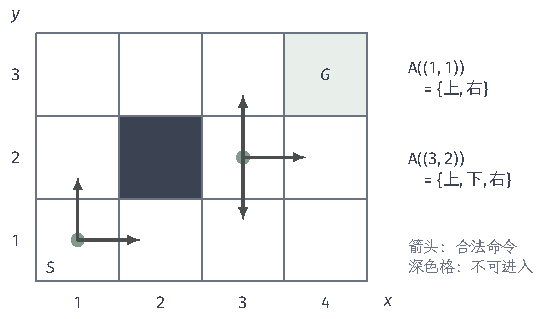
\includegraphics[width=92.019mm]{figures/07-reinforcement-learning/01-problems-and-solving/tikz/rl-overview-grid-actions.pdf}
  \caption{基准网格与两个位置的合法命令。实心方格是障碍，$S$和$G$分别表示起点与终点；箭头表示可选择的意图方向，不表示随机滑移的全部后果。}
  \label{fig:rl-overview-grid-actions}
\end{figure}

表~\ref{tab:rl-overview-action-types}按一次命令的数学形式列出输出与约束。这里的分类不涉及命令持续多久：一个持续若干步的技能仍可用离散编号或连续参数选择，只是决策时间尺度不同。这一变化由下一小节处理。

命令能够执行，也不等于执行它满足安全要求。执行器只能提供有限大小的力，是动作接口的限制；某个力在硬件上可用，却可能因碰撞风险而被禁用，则是根据行为要求进一步限制动作。两种限制可以同时进入允许集合，但安全条件怎样建立、能保证什么，需由第~\ref{chap:rl-trustworthy}章另行分析。

\begin{table}[htbp]
  \centering\small
  \begin{tabularx}{\linewidth}{@{}>{\raggedright\arraybackslash}p{19mm}*{2}{>{\raggedright\arraybackslash}X}@{}}
    \toprule
    数学形式 & 策略输出对象 & 约束接口的例子\\
    \midrule
    离散 & 一个动作编号或概率向量 & 方向掩码标出可用命令；仅对合法方向归一化\\
    连续 & 向量$\bm u$或其分布 & 力的上下界、联动约束\\
    组合 & 子集、排列或多项联合选择 & 推荐列表长度、项目去重、容量限制\\
    参数化 & 类型$c$及参数$\bm u_c$ & 不同类型有各自维度和参数范围\\
    \bottomrule
  \end{tabularx}
  \caption{动作的分类对象是一次命令的数学形式。执行器噪声属于转移机制，不会把离散命令自动变成连续动作。}
  \label{tab:rl-overview-action-types}
\end{table}

% Outline: 1.1.3.2
\subsubsection{动作后果与时间尺度}
\label{sec:rl-overview-time-scale}

在起点提交同一个向右命令，改变执行机制就会改变后果。表~\ref{tab:rl-overview-transition}固定$s=(1,1)$和命令，只对照确定移动与基准滑移。两者即时奖励都为$-0.04$，但确定移动总到$(2,1)$，随机移动还可能进入左侧竖向通道或留在起点。只看这一步的评分，就看不到后续可达区域的变化。确定移动仅是本表的对照条件，其余网格计算仍保留滑移。

\begin{table}[htbp]
  \centering\small
  \begin{tabular}{@{}lccc@{}}
    \toprule
    向右的后继状态 & 确定移动概率 & 基准概率 & 奖励\\
    \midrule
    $(2,1)$ & $1$ & $0.8$ & $-0.04$\\
    $(1,2)$ & $0$ & $0.1$ & $-0.04$\\
    $(1,1)$ & $0$ & $0.1$ & $-0.04$\\
    \bottomrule
  \end{tabular}
  \caption{同一向右命令在两种转移机制下的结果。基准的向下滑移越界，因此留在原位；零概率行仅用于对齐比较。}
  \label{tab:rl-overview-transition}
\end{table}

即使不改变机制，不同动作也可能具有相同即时奖励。在$(3,2)$选择上或下，当步都不可能到达终点，所以期望奖励同为$-0.04$。向上大概率到$(3,3)$，下一步即可尝试进入目标；向下大概率回到$(3,1)$，还需多次行动。一步评分无法表现这项差别。这里尚不声称某个动作必然最优，因为后续策略及随机转移也影响累计结果；它说明了为何需要一个跨越多步的评价对象。

动作的多步后果还要和奖励的记录时刻区分开。图~\ref{fig:rl-overview-timeline}上行沿一条可能发生的轨迹标出每次命令与反馈：执行$a_t$后得到$r_t$，而数步之后到达终点的那$1$分奖励只记录在真正到达的那一步。这就带来一个学习时无法回避的问题：当奖励很晚才出现时，应当如何用这个晚到的结果去评价早先作出的那些选择？例如终点奖励应归功于几步前那次关键转向，而不应平均分给沿途所有无关动作。这种判断哪些早先行动应对后来的收益或失败承担作用的工作，称为信用分配（credit assignment）。请注意，它改变的只是评价时如何引用历史，并不改变奖励实际发生的时间顺序——终点奖励依然发生在到达的那一刻。

\begin{figure*}[htbp]
  \centering
  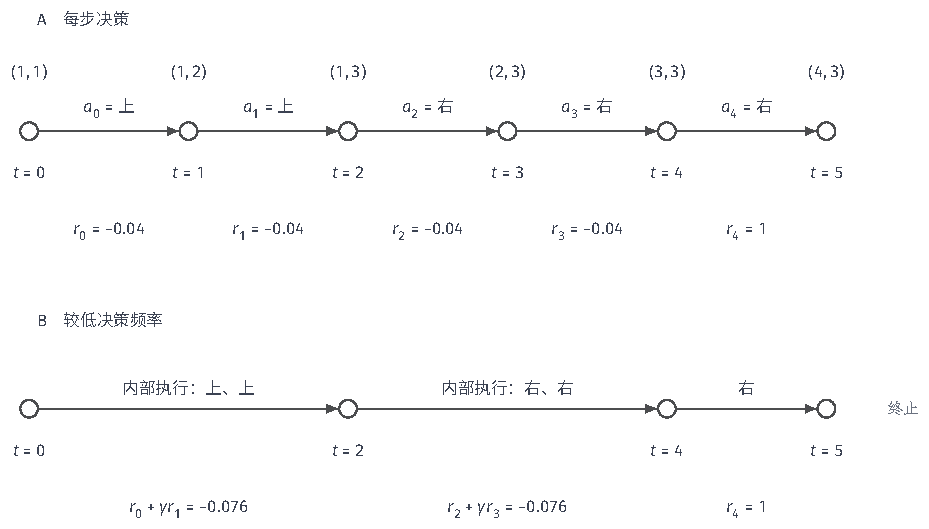
\includegraphics[width=157.371mm]{figures/07-reinforcement-learning/01-problems-and-solving/tikz/rl-overview-timeline.pdf}
  \caption{同一条五步到达轨迹的时间标记。上行每步决策，最后一个动作返回$r_4=1$；下行只在$t=0,2,4$重新决策。下行跨两步的箭头表示持有或执行内部命令的区间，不能仍用上行的一步核和单步奖励表示。}
  \label{fig:rl-overview-timeline}
\end{figure*}

图的下行改为每两步才重新决策一次。这一改变不只是少记录几个时刻：新接口下的一次动作跨过了两次原始转移，因此必须重新描述“两步之后”的状态分布，并把这期间累计的评分一并计入，不能继续套用原来的单步核和单步奖励。具体地，若一条命令持续$k$个原始步，在原始折扣$\gamma$下，区间内拿到的收益为$\sum_{j=0}^{k-1}\gamma^j r_{t+j}$；而从下一次决策时刻$t+k$才开始计算的后续累计收益，在折算回当前时刻$t$时还要整体再乘$\gamma^k$，因为它的第一项已经晚了$k$个原始步。例如两个非终止步的贡献是$-0.04+0.9(-0.04)=-0.076$，不能仍记成单个$-0.04$。若命令持续的步数本身是随机的，这段持续时间也必须作为动作后果的一部分纳入描述。

连续时间控制进一步以物理时间而非固定步号描述运动，用微分动力学或跳变机制表示变化，奖励常是单位时间的收益率。离散化时，状态变化和区间收益必须一起调整，不能只改变决策频率。本章保留这些接口区别，不把其目标混入固定步长MDP；跨步递归将在第~\ref{chap:rl-learning}章的时间抽象中展开。

% Outline: 1.1.4
\Needspace{7\baselineskip}
\subsection{策略}
\label{sec:rl-overview-policies}

% Outline: 1.1.4.1
\subsubsection{策略及其类型}
\label{sec:rl-overview-policy-types}

若网格移动没有任何误差，那么从起点依次执行“上、上、右、右、右”就能沿上路准确到达终点，此时一条事先排好的动作序列已经足够。但基准网格存在滑移：同一条命令可能把机器人带偏，一旦偏离，预先写好的余下命令就可能与当前实际位置不再匹配。这说明决策规则必须能够在行动过程中根据当前所在位置重新选择，而不是一次性写死整个动作序列。\term{策略}（policy）就是这样一条根据当前观测或决策历史选择行动的规则。此前记号$\pi(\cdot\mid s)$描述的正是它在状态$s$下给出的动作分布；某一步实际选出的$a_t$只是这条规则的一次抽样结果。

策略可以沿两个相互独立的维度变化。一个维度是规则是否随时间改变：在同一状态始终使用相同动作分布的，称为平稳策略（stationary policy）；允许这份分布随时刻变化的，称为非平稳策略（nonstationary policy）。另一个维度是给定状态后如何取值：每次只指定一个确定动作的，称为确定性策略（deterministic policy）；按一份概率分布抽样动作的，称为随机策略（stochastic policy）。这两个维度必须分别记录——是否随机抽样，与是否依赖时间并无关系，不能从一个性质推断另一个。

在有限动作情形下，固定一个状态$s$，策略给出的就是一份各动作概率组成的向量；换一个状态，这份向量可以完全不同。要把“给定状态后产生一份动作分布”的规则写到一般空间上，就使用下面的概率核记号。确定性规则把全部概率集中在同一个动作上，这种点质量分布称为Dirac分布；它仍然是一份合法的概率分布，只是取某个动作的概率为$1$，并没有改变策略作为“状态到分布的映射”这一对象类型。

\begingroup
\binoppenalty=10000
\relpenalty=10000
\begin{definition}[马尔可夫策略]
  \label{def:rl-overview-policy}
  给定状态可测空间$(S,\Sigma_S)$、动作可测空间$(\mathsf A,\Sigma_A)$及非空可测动作集合$\mathsf A(s)$。马尔可夫策略序列为$\pi=(\pi_t)_{t\geq0}$，其中每个$\pi_t(\mathrm da\mid s)$是从$S$到$\mathsf A$的概率核，并对每个$s$满足$\pi_t(\mathsf A(s)\mid s)=1$。动作有限或可数时，以$\pi_t(a\mid s)$记点质量；当$\mathbb P_\pi(s_t=s)>0$时，它等于$\mathbb P_\pi(a_t=a\mid s_t=s)$。这里的马尔可夫策略在给定$t$后只使用当前状态，不再依赖此前历史。若规则不显式依赖$t$，记为$\pi(\mathrm da\mid s)$，称为\term{平稳策略}；否则称为非平稳策略。若每个状态只输出一个合法动作$f_t(s)$，则为确定性策略；一般动作空间上对应以$f_t(s)$为原子的Dirac核，有限或可数动作下其点质量可写为$\pi_t(a\mid s)=\mathbf 1\{a=f_t(s)\}$。
\end{definition}
\endgroup

更一般的策略可以依赖全部可用历史，写成$\pi_t(\mathrm da\mid I_t)$；有限或可数动作下仍用$\pi_t(a\mid I_t)$表示点质量。本章完全可观测的主线使用上述马尔可夫策略，但不据此宣称在任何约束或观测与历史访问条件下当前状态都足够。表~\ref{tab:rl-overview-policy-types}展示抽样与时间依赖的四种组合：固定概率抽样可以是平稳的，每次确定地选择动作也可以随剩余时间改变。

\begin{table}[htbp]
  \centering\small
  \begin{tabularx}{\linewidth}{@{}>{\raggedright\arraybackslash}p{21mm}*{2}{>{\raggedright\arraybackslash}X}@{}}
    \toprule
    & 确定性 & 随机性\\
    \midrule
    平稳 & 在起点总选上 & 在起点始终以$0.7$选上、$0.3$选右\\
    非平稳 & 根据剩余步数改选近路或远路 & 剩余时间多时以$0.7$选上，少时改为$0.2$\\
    \bottomrule
  \end{tabularx}
  \caption{两种互不等同的策略属性。表中的概率是教学规则，不是估计结果；各状态仍须满足各自的动作合法性。}
  \label{tab:rl-overview-policy-types}
\end{table}

有限时域为何可能需要时间？考虑一个从导航任务简化出的独立岔路例：取消滑移和步成本，近路只需一步即以$0.4$概率得到终点奖励$1$，否则以奖励$0$终止；绕路需要两步，必得$1$。在不折扣且到时终止的规则下，只剩一步时近路期望为$0.4$、绕路为$0$；还剩两步时两者为$0.4$和$1$。同一岔路的选择随剩余时间改变。把剩余时间加入状态可以重新用平稳形式书写，但这相对于增广状态而言，并没有消除实际的时间依赖。

图~\ref{fig:rl-overview-policy-randomness}在基准起点画出两份动作概率。一份以$1$的概率选择上，另一份以$0.7$选上、$0.3$选右。即使采用第一份规则，下一状态仍以$0.8$概率为$(1,2)$、$0.1$为$(2,1)$、$0.1$留在起点。策略确定只能消除选动作时的随机性，不能消除转移随机性。状态与动作均有限的无限时域折扣MDP何时存在最优确定性平稳策略，是第~\ref{chap:rl-planning}章要证明的结论，不是策略一词本身的含义。

\begin{figure}[htbp]
  \centering
  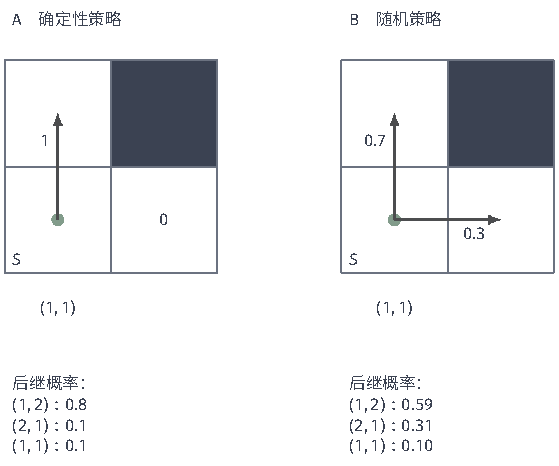
\includegraphics[width=94.580mm]{figures/07-reinforcement-learning/01-problems-and-solving/tikz/rl-overview-policy-randomness.pdf}
  \caption{同一网格起点的两种动作分布。左边确定性策略仍有随机后继；右边额外引入动作选择的随机性。图只显示起点附近，未画出的位置沿用基准网格。}
  \label{fig:rl-overview-policy-randomness}
\end{figure}

% Outline: 1.1.4.2
\subsubsection{策略诱导的轨迹与样本}
\label{sec:rl-overview-occupancy}

起点选上与选右，会把机器人带向不同区域。要计算某份策略会产生哪些训练记录，我们先求一段记录出现的概率。把包含$H$步的有限轨迹记为$\tau_H=(s_0,a_0,r_0,\ldots,s_{H-1},a_{H-1},r_{H-1},s_H)$。下面先沿有限或可数状态、动作和奖励的点质量写法计算；一般空间上的轨迹分布须逐步应用策略核与环境核，对事件作相应积分，不能把连续变量的单点概率当作密度。概率链式法则按发生顺序展开联合概率；马尔可夫性把每步环境条件缩减为当前状态动作，马尔可夫策略则给出该时刻的动作概率。因此，
\begin{equation}
  \mathbb P_\pi(\tau_H)
  =\mu_0(s_0)\prod_{t=0}^{H-1}
    \pi_t(a_t\mid s_t)\,p(s_{t+1},r_t\mid s_t,a_t).
  \label{eq:rl-overview-trajectory}
\end{equation}
初始位置来自$\mu_0$，动作来自$\pi_t$，反馈来自环境核$p$。这里使用的概率链式分解按发生顺序逐层条件化，不要求各时刻独立；同一联合律下再按中间变量取条件期望，便可把多步平均分层计算。链式分解和条件期望的迭代性质可参考\BookChapterRef{chap:random-variables}{卷2《数学准备：概率、因果与决策》中讨论随机变量的章节}。若只关心状态动作轨迹，对奖励求和后便得到含$T(s_{t+1}\mid s_t,a_t)$的乘积；不能直接把$p$替换为“奖励恒等于$R(s,a)$”。若策略依赖历史，链式分解依然成立，但动作项须改写为$\pi_t(a_t\mid I_t)$。

将这个轨迹分布记为$P_{\mathcal E}^{\pi}$；该简记还固定了奖励联合规律、观测机制与时域。本章状态完全可见，观测核为$K_o(s,\cdot)=\delta_s$。由于$o_t=s_t$，轨迹中可省写观测。部分可观测时，理论轨迹还须纳入观测机制生成的$o_0,\ldots,o_H$；实际训练记录则只能保留已经采集的字段，不能直接读出隐藏状态。

为区分这两个层次，先按理论轨迹分布生成一条轨迹，再用可测记录映射$b$保留实际可见的字段。不同的隐藏轨迹可能留下同一份可见记录；要计算某类记录出现的概率，就要把所有能生成这类记录的轨迹作为同一事件来计概率。可见记录分布记为$P_{\mathrm{rec}}^{\pi}=b_{\#}P_{\mathcal E}^{\pi}$，其中推前记号的事件读法是：对可见记录空间中的任意可测事件$C$，
\[
 P_{\mathrm{rec}}^{\pi}(C)
 =P_{\mathcal E}^{\pi}\bigl(\{\tau:b(\tau)\in C\}\bigr).
\]
右侧先在理论轨迹中找出经$b$映入$C$的全部情形，再按原轨迹分布计算这个事件的概率。本章保留可见状态时，不需要删去这些状态字段；改变观测或记录机制时，则须恢复相应依赖，不能把理论轨迹的全部状态直接当成训练记录。

沿用第~\ref{sec:rl-overview-interaction}节的三步记录，若在$(1,1)$与$(2,1)$都必选右，其概率为$0.8\times0.2\times0.8=0.128$。中间的$0.2$是两种被阻挡的滑移概率之和。只把起点改为以$0.3$概率选右，保持后两次必选右，同一记录的概率就变为$0.0384$。环境核没有改变，训练记录的分布却随策略改变了。

完整轨迹的可能种类很多，而比较不同策略会产生什么样的训练记录时，往往不必逐一罗列整条轨迹，只需知道在各个时刻、机器人有多大概率处在某些状态并采取某些动作。为此先看固定某一时刻$t$的分布，称为逐时分布（time-marginal distribution），它记录该时刻遇到各状态、各动作的概率。若还想把无限多个时刻汇总成一份分布，就必须约定不同时刻各占多大权重。由于折扣目标认为越早的后果越重要，我们自然用$\gamma^t$对逐时分布加权，再乘上$1-\gamma$使全部权重之和恰好为$1$。汇总所得的\term{折扣占用度量}（discounted occupancy measure）就是一份状态动作分布，回答这样一个问题：若按策略运行、并按这些折扣时间权重随机抽取一个时刻，那个时刻会看到什么状态、正在做什么动作。下面的$q_t^\pi(s,a)$、$d^\pi(s,a)$及求和仍采用有限或可数空间的点质量写法；一般空间上应把它们定义为状态动作集合上的测度，并将求和改为积分。

\begin{definition}[逐时分布与折扣占用度量]
  \label{def:rl-overview-occupancy}
  给定有限或可数状态动作空间上的时间齐次MDP、初始分布$\mu_0$及合法马尔可夫策略序列$\pi$。以$\mathbb P_\pi$表示它们诱导的轨迹律，逐时状态分布为$q_t^\pi(s)=\mathbb P_\pi(s_t=s)$，状态动作分布为$q_t^\pi(s,a)=q_t^\pi(s)\pi_t(a\mid s)$。对$0\leq\gamma<1$，归一化的折扣占用度量为
  \begin{equation}
    d^\pi(s,a)=(1-\gamma)\sum_{t=0}^{\infty}
      \gamma^t q_t^\pi(s,a),\qquad
    d^\pi(s)=\sum_a d^\pi(s,a).
    \label{eq:rl-overview-occupancy}
  \end{equation}
\end{definition}

我们可以把这种加权写成一次抽样：取独立于轨迹的时刻$T$，满足$\mathbb P(T=t)=(1-\gamma)\gamma^t$，则$\mathbb P_\pi(s_T=s,a_T=a)=d^\pi(s,a)$。它不是一条轨迹中“至少到访一次”的概率，反复到访与晚到访都会影响加权结果。要核对$d^\pi$确实归一化，可利用各项非负交换求和次序，再用每一时刻的概率质量为$1$：
\[
  \sum_{s,a}d^\pi(s,a)
  =(1-\gamma)\sum_{t=0}^{\infty}\gamma^t
    \underbrace{\sum_{s,a}q_t^\pi(s,a)}_{1}=1.
\]
终止后必须保留吸收状态及其虚拟动作，以上质量才仍然为$1$；若把终止后的时刻全部删除，得到的是非终止占用，其总质量一般小于$1$。吸收状态的占用高也不表示在那里继续取得奖励，因为其奖励为零。

另取只有起点$x$与吸收终点$g$的两状态教学任务，从$x$一步必到$g$，以后一直停留。取$\gamma=0.9$，只有时刻0位于$x$，因而$d(x)=0.1$、$d(g)=0.1\sum_{t\geq1}0.9^t=0.9$。两处都必定到访，至少到访一次的概率却都是1。占用描述按折扣权重抽到的时刻在哪里，不是有没有到访过；若进入$g$时奖励1、此后奖励0，回报为1，也不能把终点占用0.9当作回报。

平稳策略还满足$d^\pi(s,a)=d^\pi(s)\pi(a\mid s)$，因为每个时刻在$s$的动作分布相同。非平稳策略的占用仍由式~\eqref{eq:rl-overview-occupancy}定义，但不能把随时间变化的$\pi_t$直接提出求和号。这一区别在后续利用占用度量恢复平稳策略时会用到。

图~\ref{fig:rl-overview-occupancy}把加权分布用于比较两份完整的确定性策略。箭头给出每个非终点格的唯一意图方向，深浅及数字表示$d^\pi(s)$，不是价值。计算时先从$q_0=\mu_0$出发，对当前状态概率、动作概率和后继概率逐层加权，将分布传播到下一步：
\[
 q_{t+1}^\pi(s')=\sum_s q_t^\pi(s)
                    \sum_a\pi(a\mid s)T(s'\mid s,a)
\]
再按式~\eqref{eq:rl-overview-occupancy}累加各时刻分布。保留$400$个时刻时，总质量尾差为$0.9^{400}<5\times10^{-19}$。两幅图采用同一色标：上路策略在左侧通道的占用较大，下路策略则更多到访底边。

占用还可以联系到一项明确的记录计数协议。固定策略与初始分布，独立重复生成轨迹；每次按前述几何权重抽一个独立于轨迹的时刻，再保留该时刻的状态动作记录。若共保留$n$条这样的记录，区域$B\subseteq S$中的记录数，其期望为$n\sum_{s\in B}d^\pi(s)$。因此，在相同折扣时间权重和记录预算下，两份策略会提供不同的期望区域记录数；一份有限样本的实际计数仍有波动。这里$n$按保留的记录计数，生成这些记录消耗的真实环境交互步数须另行计算。

\begin{figure*}[htbp]
  \centering
  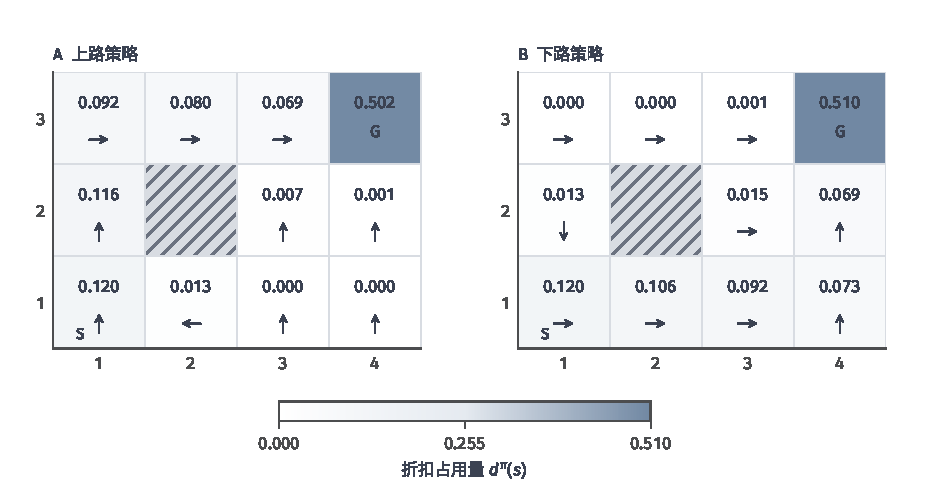
\includegraphics[width=157.400mm]{figures/07-reinforcement-learning/01-problems-and-solving/matplotlib/rl-overview-occupancy.pdf}
  \caption{基准随机网格中两份策略的归一化折扣状态占用，$\mu_0$集中于起点，$\gamma=0.9$。箭头是确定性策略，滑移仍为$0.8/0.1/0.1$；数字四舍五入至三位小数，障碍不是零概率的可用状态。}
  \label{fig:rl-overview-occupancy}
\end{figure*}

这种训练样本生成规律的差异，在“想用旧规则跑出来的经验去评价或改进一条新规则”时尤为关键，因此需要为两条规则分别命名。实际负责采集训练样本、决定日志如何产生的规则称为\termalias{rl-behavior-policy}{行为策略}（behavior policy），记为$\beta$；而我们真正想评价或改进、想知道其后果的规则称为\term{目标策略}（target policy），记为$\pi$。二者恰好相同时，称为同策略（on-policy）问题，即“用谁就评价谁”；二者不同时，称为离策略（off-policy）问题，即“用一份规则的记录去推断另一份规则”。还要注意这一划分与在线、离线的划分不同：同策略与离策略比较的是行为规则和目标规则是否为同一条，在线与离线说的则是训练过程中能否继续追加新的交互记录，两组概念互不蕴含。

用$\beta$的记录去推断$\pi$的后果，首先要检查这些记录是否覆盖了目标规则真正需要的状态和动作。如果行为分布对某个必要动作赋予的概率始终为零，那么已有样本再多，也无法靠重新加权凭空生成该动作的后果。这就是覆盖（coverage）问题：训练样本的生成规律必须为待推断的行为提供足够支持，关键不在于记录总数多，而在于关键的状态动作是否真有机会被采到。

训练样本的联合律还要由采样机制$\Gamma_{\mathrm{tr},n}$指定，不能只由单条记录分布推出。例如，从同一条长轨迹中截取相邻转移，与每次重置后独立采集完整回合，会产生不同的记录间依赖；采样机制要说明采取哪一种协议，以及每条$Z_i$保留什么。

在以固定$\beta$、按同一协议独立重复采集完整回合的基准设定中，若每条$Z_i$是一个回合的可见记录，就有$D\sim(P_{\mathrm{rec}}^\beta)^n$，右侧的幂表示$n$份回合记录的乘积分布。全部拟合与验证选择完成后，冻结最终策略$\pi$，用新的环境随机性独立运行$m$个测试回合。给定这份最终策略及固定的测试协议，便有$D_{\mathrm{te}}\sim(P_{\mathrm{rec}}^\pi)^m$；右侧是条件于所选策略后的乘积律。这里$m$是测试回合数。也可以先给定全部训练样本、验证样本和拟合与选择随机源，使最终策略固定，再说明测试回合的条件独立性；仅固定训练样本和拟合随机源，不足以排除验证选择造成的共同依赖。若只能使用旧日志，留出的评价记录仍由行为策略生成，必须通过离策略评价联系目标回报，不能假定它们已来自$\pi$。

在$(2,1)$，合法动作是左、右，两侧滑移都只会停留。若$\beta$在此永远选左，日志就没有从该格主动向右的样本，尽管$\pi$可能需要向右。另一种情况是$\beta$允许进入左侧通道，但某份有限日志恰好没到过那里。前者是行为分布本身不支持必要动作，后者可能只是有限抽样遗漏，二者不能混为同一结论。

跨位置推断可以借助函数逼近（function approximation），也就是让不同位置的预测共享参数；其可靠性仍需结构假设和相应的交互记录。网络能输出一个未尝试动作的预测，不等于该预测已被验证。占用的流守恒及由占用恢复策略将在第~\ref{chap:rl-planning}章展开，离策略覆盖的后果则由第~\ref{chap:rl-information}章进一步分析。

% Outline: 1.1.5
\subsection{奖励}
\label{sec:rl-overview-rewards}

% Outline: 1.1.5.1
\subsubsection{奖励与累计回报}
\label{sec:rl-overview-return}

策略决定怎样行动，奖励规则则决定怎样给行动后果计分。基准网格对每个非终止步收取$0.04$的代价、到达终点给$1$，这两条数值同时表达了两种偏好：希望到达目标，也希望不要拖延。但单步评分很快就不够用了：在远离终点的位置，绝大多数动作的即时奖励都是同一个$-0.04$，只比较这一个数字，根本无法区分一个动作是把机器人带向终点还是带向死路。因此评价一个动作时，必须把它之后陆续获得的奖励也一起算进来。\term{回报}（return）就是按约定的时间规则把一串奖励累计成的一个总分，用一个数概括整段行动的好坏。

沿用前面引入的折扣因子，折扣回报对$k$步之后的奖励乘权重$\gamma^k$。当$0<\gamma<1$时，越遥远的收益权重越小，这同时保证无限序列的总分通常仍是有限数；$\gamma=0$时则退化为只计当前一步。还需注意，对随机策略和随机转移而言，同一份策略可能产生许多条不同轨迹、对应许多个不同的回报实现值。本章统一按期望回报比较策略，即在同一初始分布下比较长期评分的平均值，而不是要求某条策略在每一条轨迹上都最好。

\begin{definition}[回报与策略目标]
  \label{def:rl-overview-return}
  设奖励序列$(r_t)_{t\geq0}$由给定环境和策略生成，$r_t\in\mathbb R$按执行动作的时刻编号，$0\leq\gamma<1$。若对所讨论的每个时刻$t$均有$\mathbb E_\pi\sum_{k\geq0}\gamma^k|r_{t+k}|<\infty$，从时刻$t$起的折扣回报为
  \begin{equation}
    G_t=\sum_{k=0}^{\infty}\gamma^k r_{t+k},
    \qquad 0\leq\gamma<1.
    \label{eq:rl-overview-return}
  \end{equation}
  相对于给定初始分布$\mu_0$，策略目标为$J(\pi)=\mathbb E_\pi[G_0]$。它是未归一化的期望折扣回报，不是单条轨迹的实现值。
\end{definition}

若任务只计入时刻$t$至$H-1$的奖励，且没有额外终端收益，累计范围就缩为剩余的$H-t$步：
\[
  G_{t,H}=\sum_{k=0}^{H-t-1}\gamma^k r_{t+k}.
\]
有限和允许$\gamma=1$，这时每一步权重相同。若任务持续运行，关心的是长期每步取得多少收益，则可以把前$n$步总收益除以$n$，再考察$n$增大后的极限。从状态$s$启动、遵从策略$\pi$的期望时间平均为
\[
  g^\pi(s)=\lim_{n\to\infty}\frac{1}{n}
    \mathbb E_\pi\left[\sum_{t=0}^{n-1}r_t\,\middle|\,s_0=s\right],
\]
这里须假设极限存在。该式先对随机轨迹取期望，再取时间极限；它与沿某条轨迹计算平均后得到的样本路径结论不同，本章不默认二者相等。表~\ref{tab:rl-overview-returns}比较三种累计口径，尤其要观察终止后的零奖励：它不改变奖励总和，却会被持续计入时间平均的分母。

\begin{table}[htbp]
  \centering\small
  \begin{tabularx}{\linewidth}{@{}>{\raggedright\arraybackslash}p{23mm}*{2}{>{\raggedright\arraybackslash}X}@{}}
    \toprule
    累计方式 & 权重与归一化 & 终止后怎样处理\\
    \midrule
    有限回报 & $H-t$项；$\gamma=1$时为总和而非步均值 & $H$之后不计收益；另有终端收益须显式给出\\
    折扣回报 & 权重$\gamma^k$；本书$J$不乘$1-\gamma$ & 吸收状态的零奖励不改变回报\\
    期望时间平均 & 总和除以$n$后取极限 & 终止后永远零奖励，且期望绝对累计奖励有限时，平均值为零\\
    \bottomrule
  \end{tabularx}
  \caption{回报的累计口径。对满足表中可积条件的到达任务使用无限时间平均，会失去区分路径的能力；这不是折扣回报的另一种写法。}
  \label{tab:rl-overview-returns}
\end{table}

期望时间平均中的可积条件需要控制中途部分和，不能只检查正负奖励抵消后的最终总收益。从所讨论的初态出发，若$\mathbb E_\pi\sum_{t\geq0}|r_t|<\infty$，则任意前$n$步的期望总奖励绝对值都不超过这个有限常数，除以$n$便趋于0。另一个充分条件是逐步奖励一致有界、且策略几乎必然在有限时间终止：每条轨迹的时间平均趋于0，各平均值又被同一奖励界控制，因此其期望也趋于0，不要求期望终止时间有限。基准网格的奖励有界，但仍须检查所讨论策略是否几乎必然到达终点；永远避开终点的策略不能据此得到零平均奖励结论。

\begin{example}[同一网格上的两条到达轨迹]
  \label{ex:rl-overview-path-returns}
  路径甲共五步，依次经过
  \[
    (1,1)\to(1,2)\to(1,3)\to(2,3)\to(3,3)\to(4,3).
  \]
  路径乙先从$(1,1)$到$(2,1)$再回起点，然后沿甲前进，共七步。这是两段可发生的实际轨迹，不是两种策略的全部可能结果。甲的奖励为$(-0.04,-0.04,-0.04,-0.04,1)$，乙比甲多两个前置的$-0.04$。我们固定这两串奖励，分别比较是否折扣对累计结果的影响。

  不折扣时，两者回报分别为$1-4(0.04)=0.84$和$1-6(0.04)=0.76$。取$\gamma=0.9$时，每个奖励再乘它发生时刻对应的权重：
  \[
  \begin{aligned}
    G_0^{\text{甲}}&=-0.04(1+0.9+0.9^2+0.9^3)+0.9^4\\
                  &=0.51854,\\
    G_0^{\text{乙}}&=-0.04\sum_{k=0}^{5}0.9^k+0.9^6
                    =0.3440174.
  \end{aligned}
  \]
\end{example}

绕路的回报较小，不只是因为多付了两步成本；折扣还降低了晚到的终点奖励权重。两条已发生轨迹的比较说明了累计规则，却不能直接比较两份随机策略的期望。

即时评分与累计评分甚至可以给出相反排序。另设一个确定性教学岔路：近路一步得$0.4$后终止，远路前两步得$0$、第三步得$1$，没有其他奖励。取$\gamma=0.9$，近路当前得分较高，累计回报却只有$0.4$，小于远路的$0.81$。该例取消了滑移并改变了奖励，不是原网格的计算；下一小节将保持这两条路径不变，考察折扣因子改变时排序如何变化。

有限轨迹的回报可以直接逐项相加，但无限回报首先要回答总和是否存在；实际计算时也不可能真的累加到无穷，只能保留前$H$步，因此还需知道这样截断会带来多大误差。这两个问题可以一并解决：若每步奖励的绝对值都不超过统一上界$R_{\max}$，就可以用这个奖励界乘以几何权重之和，既证明总和有限，又给出截断误差的上界。

在给定环境和策略的轨迹律下，若对所有$t$几乎处处有$|r_t|\leq R_{\max}<\infty$，且$0\leq\gamma<1$，则$\sum_{k\geq0}|\gamma^k r_{t+k}|$受几何级数$R_{\max}\sum_{k\geq0}\gamma^k$控制，因而回报绝对收敛。任意整数$H\geq1$的截断满足
\begin{equation}
 \begin{aligned}
 |G_t|&\leq\frac{R_{\max}}{1-\gamma},\\
 \left|G_t-\sum_{k=0}^{H-1}\gamma^k r_{t+k}\right|
 &\leq\frac{\gamma^H R_{\max}}{1-\gamma}.
 \end{aligned}
 \label{eq:rl-overview-tail}
\end{equation}
两项均为逐轨迹的确定上界，取条件期望后仍控制相应的期望误差；这里使用条件期望不放大确定的绝对界这一性质。绝对收敛与几何尾和可参考\BookChapterRef{chap:continuous-functions}{卷1《数学准备：计算、分析与几何》的“连续函数”章}，有界可积量的积分极限可参考\BookChapterRef{chap:measurable-functions}{卷1《数学准备：计算、分析与几何》的“可测函数”章}。给定允许误差后，第二个界可用于选择有限采集或计算的截断长度。

基准网格可取$R_{\max}=1$。只保留前$50$步时，通用尾界为$10(0.9)^{50}\approx0.05154$；这是所有满足奖励界的轨迹都适用的保守控制，不是网格的实际误差。若预先允许的误差为$\varepsilon>0$，可以反过来选择截断长度。对于$0<\gamma<1$和$R_{\max}>0$，解$\gamma^H R_{\max}/(1-\gamma)\leq\varepsilon$可得
$H\geq\log(\varepsilon(1-\gamma)/R_{\max})/\log\gamma$，
再取满足条件的正整数；分母为负，解不等式时必须改变方向。若$R_{\max}=0$，所有奖励及截断误差均为零。这些结论依赖折扣，不能用于$\gamma=1$的无限任务。

% Outline: 1.1.5.2
\subsubsection{时间目标与奖励边界}
\label{sec:rl-overview-reward-boundaries}

在前一小节的确定性岔路中，$\gamma=0.9$时远路回报更高。若更重视眼前收益，这个排序还会保持吗？我们固定近路$(0.4)$和远路$(0,0,1)$两串奖励，只改变折扣因子。该例仍没有滑移和步成本。按奖励发生的时刻加权，两条路径的回报为
\[
  G^{\text{近}}(\gamma)=0.4,\qquad
  G^{\text{远}}(\gamma)=\gamma^2.
\]
两条路径回报相等时，$0.4=\gamma^2$，故交点为$\gamma_*=\sqrt{0.4}\approx0.63246$。在这两条候选路径中，$\gamma<\gamma_*$时近路回报较高，$\gamma>\gamma_*$时远路较高，交点处相等。图~\ref{fig:rl-overview-discount}绘出的是解析函数，不是学习曲线，也没有实验误差带。把$\gamma$从$0.5$换成$0.9$后选择翻转，是目标改变的结果，不能据此判断求解算法失效。

\begin{figure}[htbp]
  \centering
  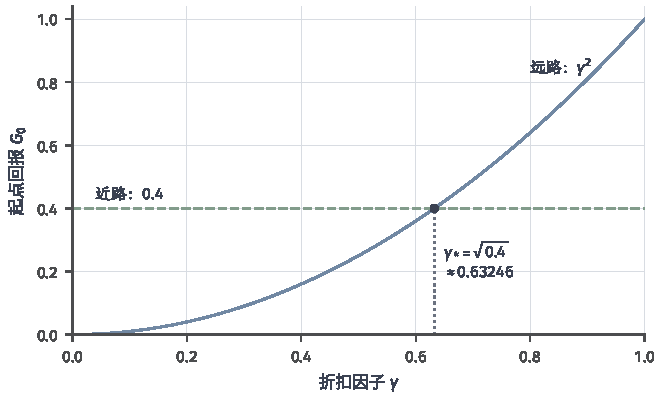
\includegraphics[width=112.000mm]{figures/07-reinforcement-learning/01-problems-and-solving/matplotlib/rl-overview-discount.pdf}
  \caption{独立确定性岔路算例的折扣偏好。横轴为$\gamma$，纵轴为起点回报；近路奖励序列为$(0.4)$，远路为$(0,0,1)$，无其他奖励。交点由解析等式求出。}
  \label{fig:rl-overview-discount}
\end{figure}

累计范围也可能因为时间上限而改变，但要先判断上限来自任务还是采集器。若任务规定“十步内到达才得分”，第十步之后的奖励不属于目标，剩余步数应作为策略可读取的状态分量，终端价值按规则设为零。若任务持续运行，只是采集器最多记录十步，$s_{10}$之后的回报并未消失。我们可以用未来价值估计补齐未记录部分，这称为自举（bootstrapping），即用已有预测代替尚未观测的后果；也可以不补齐，但需承担式~\eqref{eq:rl-overview-tail}给出的截断误差。自举不能应用于本来就不计入目标的未来。区分真正终止与采样截断，要依据任务规则，而不能只看一个含混的结束标记。

即使累计方式明确，奖励也可能鼓励我们不希望看到的行为。另设一个确定性导航任务，保留$\gamma=0.9$、原步成本和终点奖励，但增加一条两步循环。起点可以沿五步路径到达终点，也可以不断循环；到达路径不经过奖励路标，循环每步却都因经过路标多得$0.2$。循环每步净得$0.16$，无限循环的回报为$0.16/(1-0.9)=1.6$，超过五步到达的$0.51854$。这个算例取消了滑移并新增了循环，不是基准网格的精确解。选择循环可能完全符合给定奖励，却违背到达目标的意图。辅助奖励要在促进学习的同时保持最优策略不变，需要额外条件，第~\ref{chap:rl-reward}章再讨论。

奖励符合收益意图后，按期望比较仍有边界。设一个策略的回报必为$1$，另一个以各一半概率得$3$或$-1$；二者期望相同，后者却有一半概率出现负结果。平均数不能恢复失败概率、极端损失或不可违反的条件。第~\ref{chap:rl-trustworthy}章将分别讨论怎样评价回报分布、允许环境发生哪些扰动，以及行为必须满足哪些安全约束；把惩罚系数调大，不能自动给出这些保证。

% Outline: 1.1.6
\subsection{价值}
\label{sec:rl-overview-values}

% Outline: 1.1.6.1
\subsubsection{状态价值、动作价值与优势}
\label{sec:rl-overview-value-functions}

前面的轨迹算例都是在奖励串已经给定之后才算回报，但真正做决策时，我们并不知道这一步会走向哪条轨迹——既可能顺利到达，也可能因滑移偏离。要在动作尚未执行时就比较不同选择，就必须对所有可能的未来取平均。\term{价值函数}（value function）用条件期望承担这件事：固定环境、长期目标和今后遵循的策略，回答“平均而言能拿到多少回报”。这里又分两种问法。状态价值（state value）$V^\pi(s)$问的是“从状态$s$出发、包括当前动作在内都按策略$\pi$选择，平均回报是多少”；动作价值（action value）$Q^\pi(s,a)$则把当前这一步固定下来，问“从$s$出发先强制执行动作$a$、此后再按$\pi$行动，平均回报是多少”。后者专门用于比较同一个状态下的不同候选动作，因而在决策时更直接。两者之差$Q^\pi(s,a)-V^\pi(s)$称为\term{优势}（advantage），衡量“此刻特意改选动作$a$”相对于“按当前策略的平均方式行动”，平均能多拿或少拿多少回报。

\begin{definition}[状态价值、动作价值与优势]
  \label{def:rl-overview-values}
  设时间齐次MDP的奖励满足$|r_t|\leq R_{\max}<\infty$，折扣因子$0\leq\gamma<1$，$\pi$为合法平稳策略。从指定状态启动的轨迹期望定义折扣状态价值和动作价值：
  \begin{equation}
  \begin{aligned}
    V^\pi(s)&=\mathbb E_\pi[G_t\mid s_t=s],\\
    Q^\pi(s,a)&=\mathbb E_\pi[G_t\mid s_t=s,a_t=a].
  \end{aligned}
  \label{eq:rl-overview-values}
  \end{equation}
  条件事件有正概率时，以上采用通常的条件期望。对任意状态$s$，第一式按从$s$启动并遵从$\pi$定义；对任意合法动作$a$，第二式按从$s$启动、强制执行$a$、随后遵从$\pi$定义。因此，状态不必在原初始分布下可达，动作也不必满足$\pi(a\mid s)>0$。优势定义为
  $A^\pi(s,a)=Q^\pi(s,a)-V^\pi(s)$。
  有限时域或非平稳策略需要保留$V_t^\pi,Q_t^\pi,A_t^\pi$的时间下标。
\end{definition}

要从各动作的价值恢复策略在该状态的价值，需要把当前动作选择也平均进去。候选动作来自$\mathsf A(s)$，权重由固定策略给出，而不是在这里挑选最大值。下面沿有限或可数动作的点质量$\pi(a\mid s)$写成求和；一般动作空间上应改为对策略核$\pi(\mathrm da\mid s)$积分。由全期望公式，
\begin{equation}
  V^\pi(s)=\sum_{a\in\mathsf A(s)}\pi(a\mid s)Q^\pi(s,a).
  \label{eq:rl-overview-vq}
\end{equation}
优势用$V^\pi(s)$作共同基线。将其定义代入这个动作平均，再利用合法动作的概率和为$1$，得到
\[
  \sum_a\pi(a\mid s)A^\pi(s,a)
  =\sum_a\pi(a\mid s)Q^\pi(s,a)-V^\pi(s)=0.
\]
正优势表示相对于\emph{当前策略在该状态的平均行为}更好，并不表示相对于最优行为已经足够好，也不表示每次执行都会成功。

\begin{example}[随机网格中的两步价值]
  \label{ex:rl-overview-values}
  为了手算一次行动前的比较，保留基准网格全部转移与奖励，只将目标改为两步有限时域$H=2$，$\gamma=0.9$，$V_2=0$。从$c=(3,3)$开始，时刻$1$在$c$选右，在$(3,2)$选上，在$(2,3)$选右；其他状态任选合法动作，不影响以下计算。时刻$1$只剩一步，因此各处价值就是该步的期望奖励：
  \[
  \begin{aligned}
    V_1^\pi(c)&=0.792,& V_1^\pi((3,2))&=-0.04,\\
    V_1^\pi(g)&=0,& V_1^\pi((2,3))&=-0.04.
  \end{aligned}
  \]
  当前选右，以$0.8$到终点，以$0.1$留在$c$，以$0.1$到$(3,2)$。第一步期望奖励为$0.792$；第二步的期望回报按后继概率平均，再折扣一次，故
  \[
    Q_0^\pi(c,\text{右})
     =0.792+0.9[0.1(0.792)+0.1(-0.04)]=0.85968.
  \]
  当前选左时，以$0.8$到$(2,3)$，以$0.1$因向上滑移留在$c$，以$0.1$到$(3,2)$。三种后果都未到终点，所以即时期望奖励仍为$-0.04$；第二步分别使用这三个后继状态的$V_1^\pi$。

  当前选下时，以$0.8$到$(3,2)$，以$0.1$到$(2,3)$，另以$0.1$侧滑进入终点。即时奖励因而以$0.1$概率为$1$、以$0.9$概率为$-0.04$，平均为$0.064$。到终点那一支的后续价值是$V_1^\pi(g)=0$，第二步只需保留另两支的非零贡献。将各分支代入，得到
  \[
  \begin{aligned}
    Q_0^\pi(c,\text{左})
      &=-0.04+0.9[0.8(-0.04)+0.1(0.792)+0.1(-0.04)]\\
      &=-0.00112,\\
    Q_0^\pi(c,\text{下})
      &=0.1(1)+0.9(-0.04)+0.9[0.8(-0.04)+0.1(-0.04)]\\
      &=0.03160.
  \end{aligned}
  \]
  向下式中的第一个$0.9$是未进入终点的概率，方括号外的$0.9$则是折扣因子；两者数值相同，作用不同。该动作也可能因侧滑取得终点奖励，所以不能把它的即时期望误写成$-0.04$。若$\pi_0$以$0.5$选右、$0.25$选左、$0.25$选下，则
  \[
    V_0^\pi(c)=0.5(0.85968)+0.25(-0.00112)+0.25(0.03160)
              =0.43746.
  \]
  三个动作的优势依次为$0.42222,-0.43858,-0.40586$，按这些概率加权恰好为零。
\end{example}

图~\ref{fig:rl-overview-values}将这组数值放回格点，中心是当前策略的平均价值，箭头旁则是固定首动作的价值及其相对基线。只把$\pi_0$改为必选右，后续规则不变，三个$Q_0$也不变，但$V_0$变为$0.85968$。再把时刻$1$在$c$的选择改为左，就有$V_1(c)=-0.04$，当前向右的价值也变为$0.792+0.9[0.1(-0.04)+0.1(-0.04)]=0.7848$。这个对照分别改变了当前动作分布和后续策略，说明价值取决于环境、时间目标与策略，不是格子固有的属性。

\begin{figure}[htbp]
  \centering
  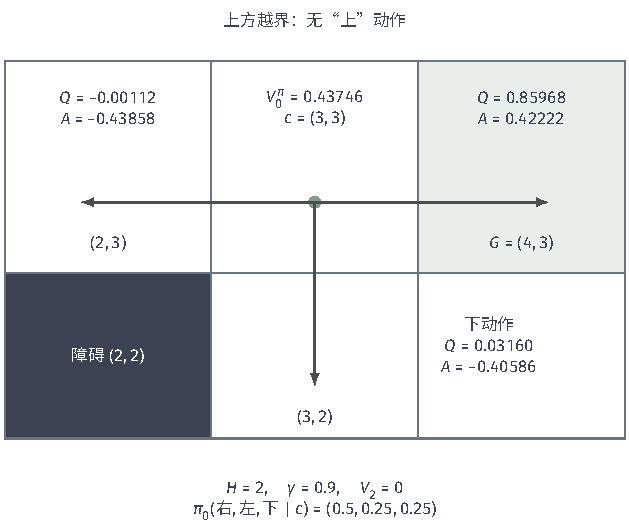
\includegraphics[width=106.581mm]{figures/07-reinforcement-learning/01-problems-and-solving/tikz/rl-overview-values.pdf}
  \caption{两步算例在$c=(3,3)$的价值分解。中心为$V_0^\pi$，三个合法意图方向标出$Q_0^\pi$与$A_0^\pi$；上方越界，因而没有上动作。全部数值对应示例~\ref{ex:rl-overview-values}，不是无限时域最优价值。}
  \label{fig:rl-overview-values}
\end{figure}

回到本章默认的无限时域折扣目标，固定时间齐次环境、合法平稳策略$\pi$与初始分布$\mu_0$，仍假设奖励有界且$0\leq\gamma<1$。在这组条件下，除按初始状态平均$V^\pi$外，还可以由策略诱导的状态动作分布计算同一个$J(\pi)$。逐时分布$q_t^\pi(s,a)$告诉我们时刻$t$遇到每种状态动作的概率，$R(s,a)$给出对应的平均奖励；两者相乘再求和，就是该时刻的期望评分。对时刻加折扣权重，便恢复总目标。有界奖励使级数绝对可和，允许交换期望与求和，得到
\begin{equation}
\begin{aligned}
  J(\pi)
   &=\mathbb E_{s_0\sim\mu_0}V^\pi(s_0)
     =\sum_{t\geq0}\gamma^t\sum_{s,a}q_t^\pi(s,a)R(s,a)\\
   &=\frac{1}{1-\gamma}\sum_{s,a}d^\pi(s,a)R(s,a).
\end{aligned}
\label{eq:rl-overview-objective-occupancy}
\end{equation}
最后一行用$d^\pi$汇总时间权重，但它比原来的折扣和多乘了$1-\gamma$，所以恢复$J$时必须除以这一系数。这把“策略去哪里、做什么”与“那些行为得到多少奖励”联系起来；后续占用分布的梯度和误差界须沿用同一归一化约定。

前面的两步算例仍使用$V_0^\pi$与有限时域回报，不能直接套用这里无时间下标的平稳价值。若要将两步任务补成无限记录，必须在第二步之后停止计奖，并保留剩余时间或相应的时间下标；这样扩展记录不会改变原来的两步目标。

% Outline: 1.1.6.2
\subsubsection{回报的递归关系}
\label{sec:rl-overview-bellman}

在两步算例中，我们先算最后一步、再把它带回当前一步。自然要问：能否用同样的“从后往前”方式处理任意长的未来，而不必逐条枚举所有轨迹？先对折扣回报本身做一次拆分。它的第一项就是当前奖励$r_t$，其余每一项都含一个共同的$\gamma$，对绝对收敛的级数可以把这个因子提到求和号外，于是得到一个不依赖任何近似的恒等式：
\begin{equation}
  G_t=r_t+\gamma G_{t+1}.
  \label{eq:rl-overview-return-recursion}
\end{equation}
有限时域下也有同样关系，只是末端为$G_{H,H}=0$。这个等式的含义很直观：从$t$起的总分，等于眼下拿到的$r_t$，加上从下一步起的总分$G_{t+1}$整体打一次折扣。恒等式本身解决了“分解”，真正的难点在于右边的$G_{t+1}$此刻尚未发生、仍是随机量，需要把它转换成可以计算的条件期望。

当前固定$s_t=s,a_t=a$后，下一步奖励和状态仍然随机。先对可能的$r_t,s_{t+1}$分情况，再评价从后继状态继续行动的回报：马尔可夫性使环境未来只依赖$s_{t+1}$，平稳策略使未来选择也只依赖后续状态。因此，
$\mathbb E_\pi[G_{t+1}\mid s_t,a_t,r_t,s_{t+1}]=V^\pi(s_{t+1})$。
先将回报分解代入动作价值，再用条件期望的塔式法则把未来回报分层平均：
\[
\begin{aligned}
 Q^\pi(s,a)
 &=\mathbb E_\pi[r_t+\gamma G_{t+1}\mid s_t=s,a_t=a]\\
 &=\mathbb E_\pi\!\left[
 r_t+\gamma\mathbb E_\pi[G_{t+1}\mid
 s_t,a_t,r_t,s_{t+1}]
 \,\middle|\,s_t=s,a_t=a\right]\\
 &=\mathbb E_\pi[r_t+\gamma V^\pi(s_{t+1})
                 \mid s_t=s,a_t=a].
\end{aligned}
\]
内层平均评价指定后继状态之后的未来，外层平均则按当前动作可能产生的奖励与后继状态计权。被替换的是$G_{t+1}$的内层条件期望，不是将每条轨迹上的随机回报都设为同一个数。有限或可数的状态与奖励下，将外层平均展开为联合概率的加权和，得到
\begin{equation}
  Q^\pi(s,a)=\sum_{s',r}p(s',r\mid s,a)
                         [r+\gamma V^\pi(s')].
  \label{eq:rl-overview-bellman-qv}
\end{equation}
该式把当前动作的价值变成一步反馈与后继状态价值的平均。用式~\eqref{eq:rl-overview-vq}平均当前动作，可得到$V^\pi$的递推；用同一式替换后继$V^\pi$，可得到$Q^\pi$的递推。

两式称为\term{Bellman期望关系}（Bellman expectation equations），它们都在评价固定策略，平均权重来自策略与环境，而不是对动作求最优：
\begin{align}
 V^\pi(s)
  &=\sum_a\pi(a\mid s)
        \left[R(s,a)+\gamma\sum_{s'}T(s'\mid s,a)V^\pi(s')\right],
        \label{eq:rl-overview-bellman-v}\\
 Q^\pi(s,a)
  &=R(s,a)+\gamma\sum_{s'}T(s'\mid s,a)
          \sum_{a'}\pi(a'\mid s')Q^\pi(s',a').
        \label{eq:rl-overview-bellman-q}
\end{align}
从联合核改写成$T,R$时，分别平均$r_t$和后继价值，只使用了期望的线性性，不要求二者独立。网格奖励恰好由后继状态决定，仍可使用这两式。递推现在给出了计算关系，但还需核对它计算的确实是原来定义的回报期望。有限时域可以从零终端值逐步往前验证；无限时域则需用尾项界控制有限截断与完整回报的差。

\begin{theorem}[回报期望与递推一致]
  \label{thm:rl-overview-recursion}
  设MDP的状态与动作均有限，各允许动作集合非空，$\pi$为合法马尔可夫策略序列。给定整数时域$H\geq1$及$0\leq\gamma\leq1$，每个时刻、每个合法状态动作的奖励绝对可积，终端价值为零。按$V_H^\pi=0$及
  \begin{equation}
    V_t^\pi(s)=\sum_a\pi_t(a\mid s)
      \int_{S\times\mathbb R}
      [r+\gamma V_{t+1}^\pi(s')]
      p_t(\mathrm d s',\mathrm d r\mid s,a)
    \label{eq:rl-overview-finite-recursion}
  \end{equation}
  反向计算，得到的量等于$\mathbb E_\pi[G_{t,H}\mid s_t=s]$。这里允许环境核$p_t$随时刻变化；时间齐次时$p_t=p$。
  对时间齐次模型、固定平稳策略、有界奖励与$0\leq\gamma<1$，无限折扣回报的条件期望满足式~\eqref{eq:rl-overview-bellman-v}和式~\eqref{eq:rl-overview-bellman-q}。
\end{theorem}

\begin{proof}
  与价值定义相同，零概率条件事件处采用从指定状态启动的含义。有限时域在$t=H$无剩余奖励，两边都为零。假设时刻$t+1$的递推值已经等于剩余回报的条件期望。将$G_{t,H}=r_t+\gamma G_{t+1,H}$代入，再按动作、奖励和后继状态逐层取条件期望，得到
  \[
  \begin{aligned}
   &\mathbb E_\pi[G_{t,H}\mid s_t=s]\\
   &\quad=\sum_a\pi_t(a\mid s)
      \int_{S\times\mathbb R}
      \bigl[r+\gamma\mathbb E_\pi[G_{t+1,H}\mid s_{t+1}=s']\bigr]\\
   &\qquad\qquad{}\times p_t(\mathrm d s',\mathrm d r\mid s,a).
  \end{aligned}
  \]
  内层条件期望只需$s_{t+1}$，是因为模型在给定时刻满足马尔可夫性，未来采用指定的策略序列。代入归纳假设就得到式~\eqref{eq:rl-overview-finite-recursion}。由$t=H-1$逐次归纳到$t=0$，有限结论成立。固定当前动作而不平均$\pi_t$，同一论证给出有限时域的$Q_t^\pi$关系。

  对无限折扣情形，令$V^{\pi,[n]}(s)$为从$s$开始只累加前$n$步的回报期望，方括号表示截断长度而非更新迭代。由已经证明的有限结论，
  \[
    V^{\pi,[n]}(s)=\sum_a\pi(a\mid s)
       \left[R(s,a)+\gamma\sum_{s'}T(s'\mid s,a)
                                       V^{\pi,[n-1]}(s')\right].
  \]
  式~\eqref{eq:rl-overview-tail}给出对所有$s$一致的界
  $|V^{\pi,[n]}(s)-V^\pi(s)|\leq\gamma^nR_{\max}/(1-\gamma)$，
  因而左边收敛到$V^\pi(s)$。右边加权平均的差至多为
  $\gamma\cdot\gamma^{n-1}R_{\max}/(1-\gamma)$，也趋于零，故极限满足式~\eqref{eq:rl-overview-bellman-v}。对固定首动作的截断回报重复同样步骤，得到式~\eqref{eq:rl-overview-bellman-qv}；再用动作平均关系替换其中的$V^\pi$，即得到式~\eqref{eq:rl-overview-bellman-q}。
\end{proof}

证明从回报定义出发，先验证有限递推，再用尾项界过渡到无限回报，因此没有用递推本身假定价值存在。但“价值满足这些式子”还不能反过来说明只有这一个函数满足它们，也不能说明反复计算右侧会收敛。不动点唯一性与计算误差由第~\ref{chap:rl-planning}章补足。

图~\ref{fig:rl-overview-backup}将式中的两层平均分开：先按策略选择动作，再按环境生成后继。若不再按当前策略平均，而是在合法动作中选择期望累计回报最大的一个，问题就从评价这份策略转为改进行为。最大值的候选集合是$\mathsf A(s)$，比较指标是动作的期望回报；这一新的求解问题也由规划章展开。

\begin{figure}[htbp]
  \centering
  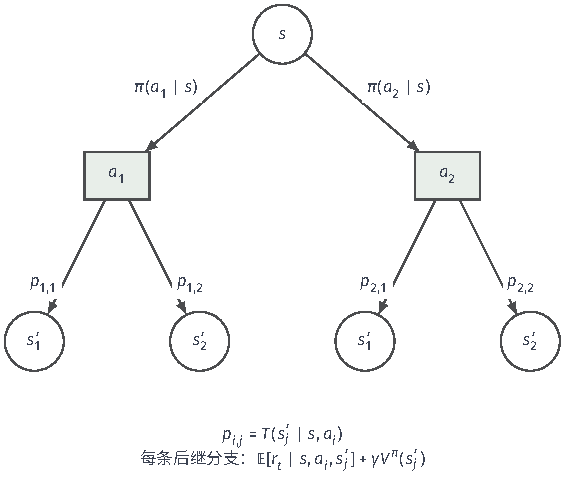
\includegraphics[width=95.617mm]{figures/07-reinforcement-learning/01-problems-and-solving/tikz/rl-overview-backup.pdf}
  \caption{Bellman期望备份的两层随机性。圆节点表示状态，方节点表示动作；第一层以$\pi(a\mid s)$平均，第二层以$T(s'\mid s,a)$平均后继价值。给定状态动作的即时奖励平均为$R(s,a)$；若按后继分支同时计入奖励，需保留奖励与后继状态的条件关系。}
  \label{fig:rl-overview-backup}
\end{figure}

% Outline: 1.2
\section{强化学习的研究内容}
\label{sec:rl-overview-research}

同一个网格任务可以提出不同问题：已有策略的回报怎样，怎样找到更好的策略，以及应当去哪里收集训练样本。回答这些问题，需要同时说明求解目标、环境访问权限和评价依据。

% Outline: 1.2.1
\subsection{核心研究问题}
\label{sec:rl-overview-questions}

给定一份策略，估计它的长期回报，称为\term{策略评价}（policy evaluation）；选择或改进策略以提高期望回报，称为\term{控制}（control）。当环境规律未知时，还需要\term{探索}（exploration）：主动尝试动作，取得能够区分候选动作后果的训练样本。探索可能牺牲当前回报，换取以后作出更好决策的依据。

求解可以沿两条路线进行。基于模型（model-based）方法显式利用环境的转移与奖励规律；规律未知时，先从交互记录估计环境模型，再据此规划。无模型（model-free）方法直接从训练样本估计价值或调整策略。这里的“模型”特指预测环境后果的模型，因此用神经网络表示价值函数仍可以是无模型方法。

图~\ref{fig:rl-overview-research-flow}展示这些路线怎样接入交互过程。价值估计帮助改进策略，环境模型支持预测与规划，新策略又改变后续训练样本的分布。晚到的奖励怎样评价早先动作、怎样表示复杂观测，以及更新能否稳定，都是这些路线共同面对的问题。

\begin{figure}[htbp]
  \centering
  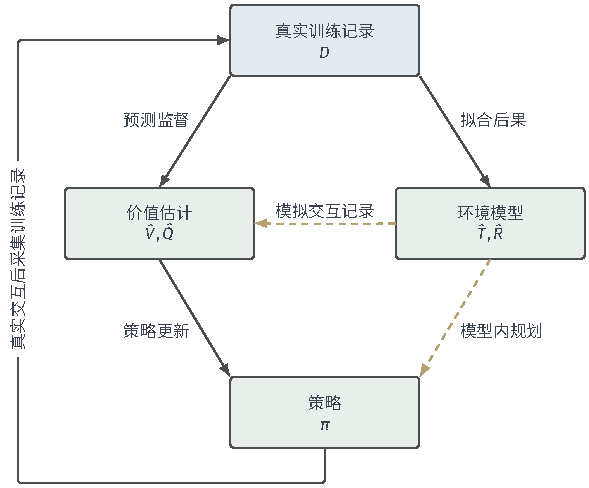
\includegraphics[width=99.815mm]{figures/07-reinforcement-learning/01-problems-and-solving/tikz/rl-overview-research-flow.pdf}
  \caption{训练样本、价值估计、环境模型与策略之间的依赖。实线表示真实交互记录参与模型拟合、价值估计及策略更新；虚线表示利用学习模型规划或生成模拟交互记录。各条路线可以组合使用。}
  \label{fig:rl-overview-research-flow}
\end{figure}

% Outline: 1.2.2
\subsection{问题边界与变体}
\label{sec:rl-overview-protocols}

环境模型是否已知，首先决定了求解任务。转移与奖励规律已知时，主要困难是在多步选择中控制计算量和近似误差，第~\ref{chap:rl-planning}章介绍动态规划与搜索。规律未知时，还需从有限训练样本估计动作后果，并协调探索与策略改进，第~\ref{chap:rl-learning}章介绍蒙特卡罗、时序差分、策略梯度和环境模型学习。

模型未知时，训练样本的采集权限也有不同设定。在线学习通常要沿实际轨迹到达某个状态，才能尝试该处的动作；\term{生成模型}（generative model）允许指定合法状态动作对，查询随机后继状态和奖励样本；离线学习只能使用固定日志。随机查询不等于知道精确转移概率，在线交互也不自动允许任意重置。有限批次交互则只在规定轮次内追加训练样本。

模型与采集权限之外，观测、奖励和任务要求也会改变问题。表~\ref{tab:rl-overview-variants}列出主要设定及后续章节的处理路线。观测不完整造成的是当前状态难以辨认，固定日志造成的是部分动作后果缺少训练样本，两者需要分别处理。

\begin{table*}[htbp]
  \centering\small
  \begin{tabularx}{\linewidth}{@{}>{\raggedright\arraybackslash}p{24mm}*{2}{>{\raggedright\arraybackslash}X}@{}}
    \toprule
    问题设定 & 主要困难 & 方法与承接位置\\
    \midrule
    观测不完整 & 同一观测可能对应不同状态，单次观测可能遗漏决策依据 & 根据交互历史推断状态，利用记忆或主动探测；第~\ref{chap:rl-information}章\\
    训练样本固定 & 待评价或改进的策略可能选择日志未覆盖的动作，无法补采其后果 & 离策略评价、行为约束与保守价值估计；第~\ref{chap:rl-information}章\\
    缺少可信奖励 & 缺少可信的标量奖励反馈，示范或偏好也未必唯一确定目标 & 行为克隆、逆强化学习、奖励建模与反馈校验；第~\ref{chap:rl-reward}章\\
    任务发生变化 & 目标、动力学或观测机制改变，旧策略未必仍然适用 & 共享表示、任务推断与元学习；第~\ref{chap:rl-transfer}章\\
    多个决策者 & 动作后果取决于共同选择，其他参与者也可能在学习 & 联合决策建模、集中训练与分散执行、自我对弈；第~\ref{chap:rl-multi-agent}章\\
    风险或安全受限 & 平均回报之外，还需控制严重失败、动力学扰动下的回报损失与约束违反 & 风险敏感优化、鲁棒规划、约束优化与安全过滤；第~\ref{chap:rl-trustworthy}章\\
    \bottomrule
  \end{tabularx}
  \caption{强化学习的主要问题变体。各行改变不同条件，可以在同一任务中同时出现；相应方法的保证仍依赖具体的观测、训练样本覆盖和环境假设。}
  \label{tab:rl-overview-variants}
\end{table*}

奖励受限还需区分两种情形。已经观测到随机奖励、只是其均值未知，属于通常的未知模型设定。\term{奖励无关探索}（reward-free exploration）则先在不知道奖励函数时收集转移记录，之后取得完整且有界的奖励函数，再用这些固定记录规划，不再追加交互。它要为全部允许的后续奖励保留足够覆盖，与从示范或偏好中学习奖励不同；相关协议见第~\ref{sec:rl-learning-guarantees-access}节。

这些设定可以叠加。例如，机器人可能只看到局部货架，只能用旧仓库日志训练，到新仓库后还须与其他机器人协作并避免碰撞。组合方法时，需要重新核对每一种限制下的适用条件。

% Outline: 1.2.3
\subsection{评价与研究证据}
\label{sec:rl-overview-evidence}

评价应与研究目标对应。价值估计关注预测与真实价值的误差，控制关注策略的期望回报，探索还需计入收集训练样本的代价。减少真实交互次数可能需要更多模型内计算，因此真实环境转移次数、模型查询次数与计算时间应分别报告。

评价训练完成后的策略时，应先固定策略和测试协议，再用未参与训练与候选选择的独立评价样本估计回报。任务目标、评价初始分布和时间范围必须一致。多个评价回合反映同一策略回报的随机波动，多次独立训练则反映学习过程的波动；两者都需要报告。任务外泛化还应单列新任务的适应预算，安全研究则需另报失败或约束违反情况。

定理说明假设成立时可以保证什么，受控实验考察具体设置下的方法作用，跨任务评价检验结果能延伸到哪些任务。三类证据相互补充，结论都应保持在各自的假设与评价范围内。

% Outline: 1.3
\section{强化学习的研究历史}
\label{sec:rl-overview-history}

强化学习逐步连接了三个问题：怎样根据结果改变行为，怎样规划多阶段行动，以及怎样从连续经验学习长期预测。随着表示能力和计算规模扩大，研究又进入高维观测、连续控制和更复杂的交互设定。

% Outline: 1.3.1
\subsection{强化学习的思想源流}
\label{sec:rl-overview-origins}

一种行为得到某种结果后，以后还会不会再被选择？Thorndike在早期行为研究及1911年的专著中讨论效果律（law of effect），将情境、行为与后果联系起来，为试错学习提供了思想线索。当时尚无本章的MDP与折扣目标框架\scite{rl1-thorndike1911-learning}。

动态与目标已知时，困难在于怎样安排一系列行动。Bellman的动态规划把长期决策分解为后继子问题，用后继价值比较当前选择，建立了递归求解的基础\scite{rl1-bellman1957-dp}。对于从经验改善预测的问题，Samuel的跳棋程序探索了局面评价的学习；程序仍利用已知棋局规则与搜索\scite{samuel1959}。

终局结果出现很晚时，还可以利用相邻时刻的预测来学习。Sutton在1988年的工作中系统讨论\term{时序差分}（temporal difference, TD）预测，用一步奖励和后继价值预测修正当前预测，使长期评价可以逐步更新\scite{rl1-sutton1988-td}。图~\ref{fig:rl-overview-history}将这些线索及相关代表工作放在同一时间线上。

\begin{figure*}[htbp]
  \centering
  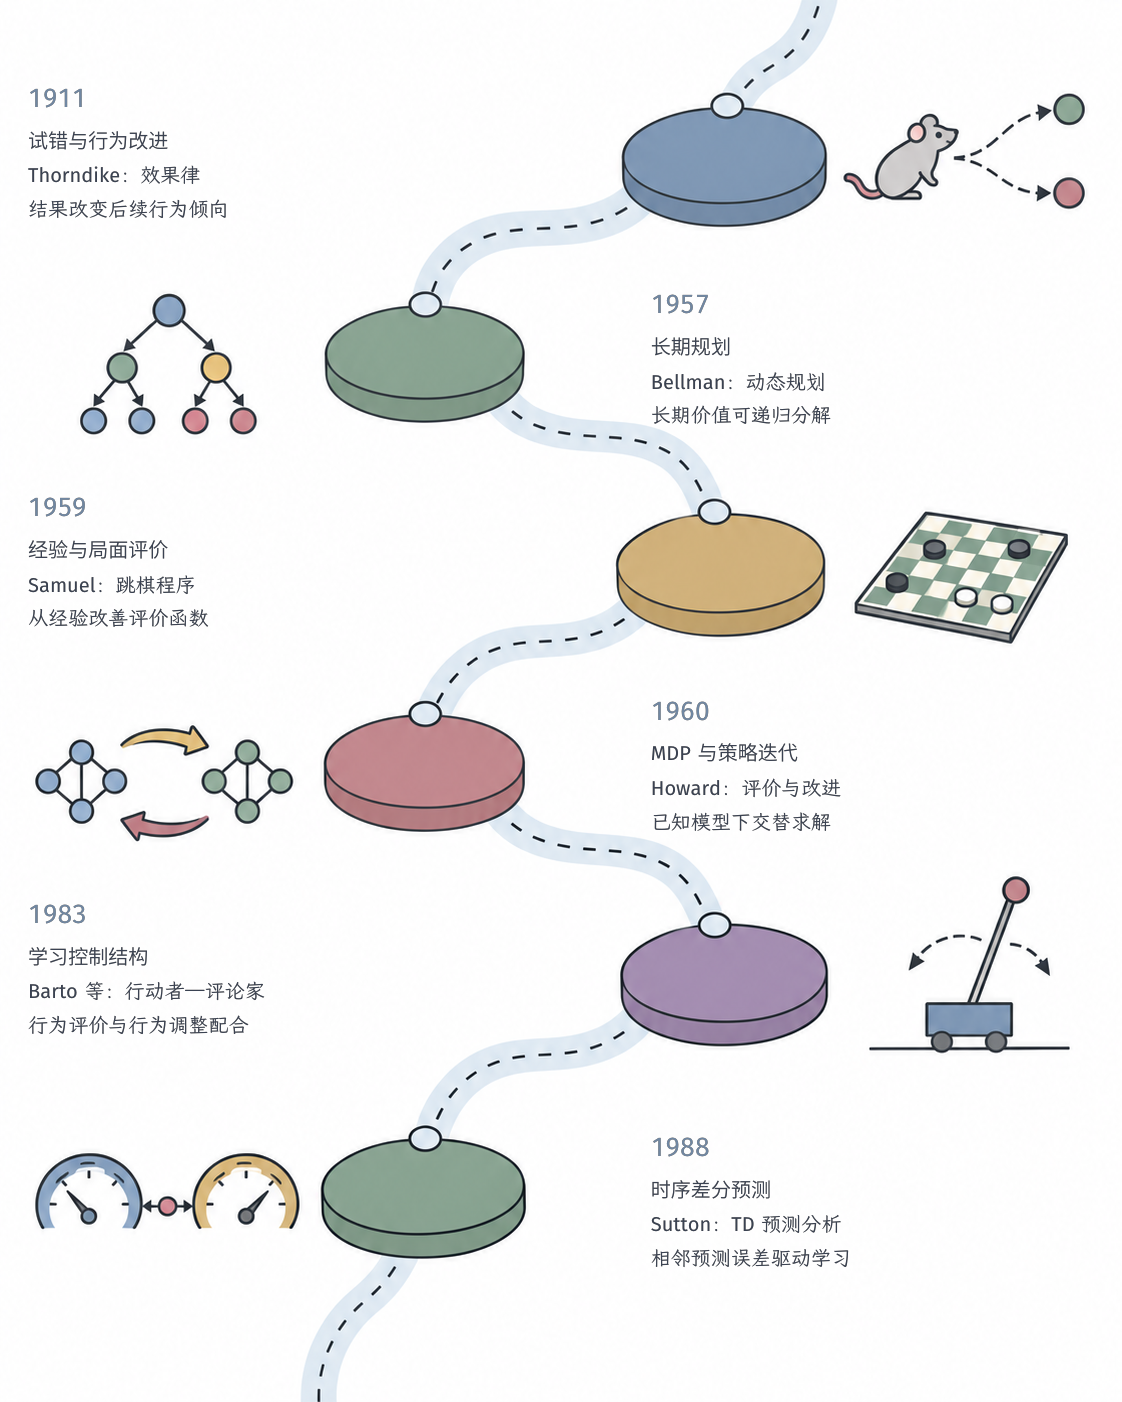
\includegraphics[width=157.400mm,height=.88\textheight,keepaspectratio]{figures/07-reinforcement-learning/01-problems-and-solving/generated/rl-overview-history/figure.png}
  \caption{强化学习思想源流的代表工作。沿曲线路径从上向下按年代阅读，节点间距不按年份等比例缩放；年份对应正文所引代表文献，路径不表示直接因果继承或方法替代。}
  \label{fig:rl-overview-history}
\end{figure*}

% Outline: 1.3.2
\subsection{现代强化学习框架的形成}
\label{sec:rl-overview-modern}

MDP使已知模型下的规划与未知模型下的学习能够围绕同一长期目标讨论。Howard在1960年的专著中系统发展了MDP的动态规划与策略迭代，交替评价当前策略并据此改进，形成了已知模型下的重要求解路线\scite{rl1-howard1960-dp}。

模型未知时，蒙特卡罗评价用采样回报估计价值，TD则利用一步经验和已有预测构造更新目标。前者在有限时域任务中可以等到轨迹结束，后者缩短了等待，但目标也受价值预测误差影响。把评价接到行为调整上，\term{行动者—评论家}（actor--critic）让评论家估计长期后果，再据此更新行动者的动作分布；Barto、Sutton与Anderson在1983年的学习控制工作中研究了这种配合结构\scite{rl1-barto1983-control}。

Q-learning直接估计最优动作价值，通过比较后继状态的候选动作来形成学习目标。Watkins于1989年提出该方法，Watkins与Dayan在1992年给出限定条件下的收敛证明，条件包括表格表示、充分访问和适当步长\scite{rl1-watkins1992-qlearning}。这些方法将价值学习与行为改进连接起来，具体更新及其成立条件见第~\ref{chap:rl-learning}章。

% Outline: 1.3.3
\subsection{函数逼近与规模扩展}
\label{sec:rl-overview-approximation}

连续位置、速度和关节角无法逐点存入价值表，高维离散状态的组合数也会迅速增长。函数逼近用共享参数计算价值或动作分布，使有限训练样本能够影响多个状态的预测。近似动态规划研究怎样在这种受限表示下计算价值并改进策略，Bertsekas与Tsitsiklis的神经动态规划专著系统连接了动态规划、仿真与函数逼近\scite{rl1-bertsekas1996-ndp}。

策略也可以直接用参数表示，再沿期望回报上升的方向调整参数，这就是策略梯度的基本思路。Williams在1992年研究的REINFORCE用采样回报加权动作对数概率的导数，估计策略梯度，无须对环境动态求导；这类估计的抽样波动也推动了后续的方差控制研究\scite{rl1-williams1992-reinforce}。

参数共享带来泛化，也带来状态间的相互干扰。利用后继预测修正当前预测称为自举，使用其他策略采集的训练样本学习称为离策略学习。函数逼近与这两种机制结合时，更新可能发散，表格方法的收敛结论不能直接推广到任意网络。第~\ref{chap:rl-learning}章将展开这些机制及稳定学习的条件。

% Outline: 1.3.4
\subsection{深度强化学习的兴起}
\label{sec:rl-overview-deep}

根据游戏画面选择动作，需要同时学习观测表示与长期价值。深度Q网络（deep Q-network, DQN）将卷积网络与动作价值学习结合，并用经验回放复用交互记录、用目标网络减缓学习目标的变化。2015年的Atari游戏结果展示了这种组合处理高维视觉观测的能力\scite{mnih2015}。

连续控制难以枚举全部候选动作。深度确定性策略梯度（deep deterministic policy gradient, DDPG）用行动者直接给出连续动作，再由评论家估计动作价值并指导行动者更新，将深度方法扩展到模拟物理控制\scite{rl1-lillicrap2016-ddpg}。

对于规则已知、可进行前瞻模拟的围棋，AlphaGo的2016年系统结合策略网络、价值网络与蒙特卡罗树搜索，用模拟对局分配搜索预算，以网络指导候选落子和局面评价，并通过人类棋谱及自我对弈训练\scite{silver2016}。这些进展分别利用了表示学习、策略优化和搜索；游戏或仿真中的成功仍须结合相应的模型访问与交互条件理解。

% Outline: 1.3.5
\subsection{研究范围的拓展}
\label{sec:rl-overview-expansion}

研究也逐步处理完整状态与可信奖励难以取得的任务。部分可观测决策根据历史观测推断隐藏状态，Kaelbling、Littman与Cassandra在1998年的工作系统讨论了相应规划框架\scite{rl1-kaelbling1998-pomdp}。目标难以直接写成奖励时，则可利用示范或人类反馈；Christiano等在2017年用人类对轨迹片段的偏好训练奖励预测，再据此学习策略\scite{christiano2017}。

多个决策者与行为约束也有长期研究基础。Shapley在1953年研究随机博弈，将状态转移与多个参与者的共同决策联系起来；约束MDP则在回报目标之外另设成本预算，Altman的专著系统处理了这类问题\scite{rl1-shapley1953-games,rl1-altman1999-cmdp}。这些方向改变的是观测、目标或参与者等问题条件，其方法与后文章节的对应关系已在表~\ref{tab:rl-overview-variants}中列出，并不构成深度强化学习之后才依次出现的年代阶段。

% Outline: 1.3.6
\subsection{前沿研究方向}
\label{sec:rl-overview-frontiers}

跨任务研究希望复用已有训练结果，减少新任务所需的训练样本。Gato用统一序列组织多种任务的观测和动作编码，通过监督式序列训练学习共享参数\scite{rl1-reed2022-gato}。共享编码仍需对齐具体任务的观测与动作含义，不能使不同机器人的动作编号自动互换。

进一步的上下文强化学习把已有或新增的观测、动作和奖励记录作为决策依据，在参数固定时调整后续行为。可扩展上下文Q学习（S-ICQL）从这些交互记录估计动作价值，再据此生成策略，Vintix II研究多领域决策预训练及上下文适应\scite{rl1-liu2026-sicql,rl1-polubarov2026-vintix}。在线适应可以取得新反馈，离线推断只能使用给定记录；两者的交互预算与适用任务范围需要分别评价，相关机制见第~\ref{chap:rl-transfer}章。

另一条路线先学习可供决策使用的\term{世界模型}（world model），即根据观测和给定动作预测后继变化与任务反馈的环境模型。DreamerV3在模型预测的想象轨迹中训练策略，TD-MPC2在每次决策时利用学习模型规划，Dreamer 4探索由固定离线记录训练模型并在模型内学习行为\scite{rl1-hafner2025-dreamerv3,rl1-hansen2024-tdmpc2,rl1-hafner2025-dreamer4}。图~\ref{fig:rl-overview-world-loop}展示模型内求解怎样接回真实环境：预测轨迹中的高回报仍需真实评价，旧轨迹上的预测准确也不保证未尝试动作的后果预测准确。

\begin{figure}[htbp]
  \centering
  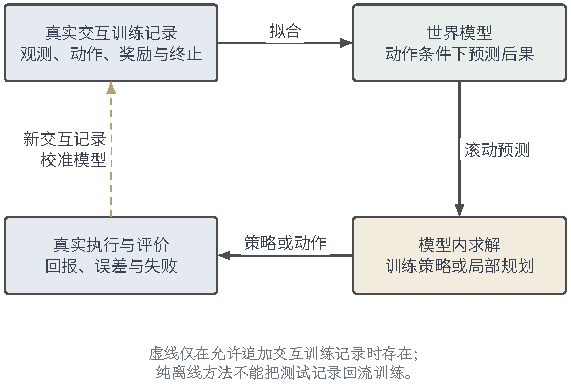
\includegraphics[width=96.615mm]{figures/07-reinforcement-learning/01-problems-and-solving/tikz/rl-overview-world-loop.pdf}
  \caption{可供决策使用的世界模型闭环。实线连接训练样本、模型内求解与独立评价；虚线校准路径只在允许追加真实训练记录时存在。模型预测的回报需要在真实环境中检验。}
  \label{fig:rl-overview-world-loop}
\end{figure}

工具使用把动作扩展为检索、运行程序或修改文件等调用，面临长程信用分配和局部观测的困难。Agent Lightning将执行程序与策略训练分开，保存实际调用记录，再据此更新语言模型策略；其后续版本进一步对齐训练采样与实际运行流程\scite{rl1-luo2025-lightning,rl1-he2026-lightning}。一次工具调用与语言模型生成的一个词元对应不同的动作尺度，任务成功率也须在相同工具权限和调用预算下比较。

要进一步回答“若主动改选动作会怎样”，还需要区分预测与因果识别。观察日志中的关联未必确定干预结果，即使各动作的转移分布已知，也未必能够回答同一次具体经历若换一个动作会怎样；相关区分可参考\BookChapterRef{chap:causal-inference}{卷2《数学准备：概率、因果与决策》中讨论因果响应的章节}。Oberst与Sontag用结构因果模型构造反事实轨迹，所得解释依赖所指定的生成机制\scite{rl1-oberst2019-counterfactual}。跨任务复用这类机制时，还须明确哪些关系保持不变，以及已有观察或干预记录是否足以确定所求结果。

% Outline: 1.4
\section{本章小结}
\label{sec:rl-overview-summary}

回到网格任务，决策问题现在有了可核算的说明。状态是除障碍外的格子，合法命令按意图方向确定，环境以$0.8/0.1/0.1$执行或滑移；起点、终点吸收与奖励规则固定。给出一份策略，就能由动作概率与环境核计算轨迹概率，再用占用度量汇总折扣时间中的状态动作分布。回报给这些轨迹计长期总分，价值则在行动前按可能后果取平均。策略改变的既是长期回报，也是后续经验的来源。

章首的机器人因此不能只按当前距离选择动作：距离变小，并不能保证整段行动到达目标，更不能保证安全。比较行动需指定后继分布、长期评分和后续规则；从经验作出比较，还需检查训练样本是否覆盖待选行为的后果。本章给出了描述和评价这些关系的对象，尚未求出仓储任务的最优安全路线。表~\ref{tab:rl-overview-distinctions}用三个具体判断收拢易混对象，便于继续检查求解方法与实验结论。

\begin{table*}[htbp]
  \centering\small
  \begin{tabularx}{\linewidth}{@{}>{\raggedright\arraybackslash}p{31mm}>{\raggedright\arraybackslash}X@{}}
    \toprule
    区别 & 可用于检验理解的具体判断\\
    \midrule
    状态与观测 & 相同照片可能对应门已开或未开；照片不一定是充分状态。见第~\ref{sec:rl-overview-mdp}节。\\
    奖励样本与长期价值 & $(3,3)$向右的一次奖励是$1$或$-0.04$；两步$Q_0^\pi=0.85968$是多种未来的平均。见第~\ref{sec:rl-overview-value-functions}节。\\
    行为与目标策略 & 日志始终向左，不代表待评价策略也应向左；右行的后果仍可能缺证据。见第~\ref{sec:rl-overview-occupancy}节。\\
    \bottomrule
  \end{tabularx}
  \caption{对象不同，能够回答的问题也不同。数值判断沿用本章明确给出的两步算例，不能移作无限时域结论。}
  \label{tab:rl-overview-distinctions}
\end{table*}

有界奖励与$0\leq\gamma<1$保证了折扣回报存在，也给出截断尾项界；有限时域和无限折扣下的条件期望论证则说明价值满足递推。价值存在和满足递推，还不意味着已经有可承受的求解方法，也不意味着有限训练样本能估计得足够准。第~\ref{chap:rl-planning}章先在模型可访问时建立规划与计算误差基准，区分精确期望和指定查询点的随机采样；第~\ref{chap:rl-learning}章再处理未知环境中的经验收集、估计与策略改进。历史和前沿中的方法虽然扩展了表示与接口，结论仍须绑定评价目标、观测机制和训练样本采集权限，因为行动始终同时改变结果与学习证据。
